
% !TEX encoding = UTF-8 Unicode
% !program = pdflatex

\documentclass[a4paper,11pt]{article}
\usepackage[a4paper,top=38mm,right=16mm,bottom=24mm,left=25mm,head=35mm,foot=15mm]{geometry}
\usepackage[comma]{natbib}
\bibliographystyle{agsm}
\usepackage[english]{babel}
\usepackage{tocbibind}
\usepackage{makecell}

% font
\usepackage[utf8]{inputenc}
\usepackage{graphicx}
\graphicspath{ {images/} }
\usepackage[T1]{fontenc}
\usepackage[parfill]{parskip}
\usepackage{soul,rotating}
\usepackage{pdflscape}

\usepackage{helvet}
\renewcommand*\familydefault{\sfdefault}


% syntax highlighting of code
\usepackage{listings}
\usepackage{color}
\definecolor{gray}{rgb}{0.4,0.4,0.4}
\definecolor{darkblue}{rgb}{0.0,0.0,0.6}
\definecolor{cyan}{rgb}{0.0,0.6,0.6}

\lstset{
  basicstyle=\ttfamily,
  columns=fullflexible,
  showstringspaces=false,
  commentstyle=\color{gray}\upshape
}

\lstdefinelanguage{XML}
{
  numbers=left,
  numberstyle=\scriptsize,
  morestring=[b]",
  morestring=[s]{>}{<},
  morecomment=[s]{<?}{?>},
  stringstyle=\color{black},
  identifierstyle=\color{darkblue},
  keywordstyle=\color{cyan},
  frame=lines,
  morekeywords={xmlns,version,type,rdf,fam}
}

\lstdefinelanguage{GraphQL}
{
  numbers=left,
  numberstyle=\scriptsize,
  morestring=[b]",
  morestring=[s]{>}{<},
  morecomment=[s]{<?}{?>},
  stringstyle=\color{black},
  identifierstyle=\color{darkblue},
  keywordstyle=\color{cyan},
  frame=lines,
  morekeywords={xmlns,version,type,rdf,fam}
}

\lstdefinelanguage{JSON}{
    numbers=left,
    numberstyle=\scriptsize,
    stepnumber=1,
    numbersep=1pt,
    showstringspaces=false,
    breaklines=true,
    frame=lines,
    literate=
     *{0}{{{\color{cyan}0}}}{1}
      {1}{{{\color{cyan}1}}}{1}
      {2}{{{\color{cyan}2}}}{1}
      {3}{{{\color{cyan}3}}}{1}
      {4}{{{\color{cyan}4}}}{1}
      {5}{{{\color{cyan}5}}}{1}
      {6}{{{\color{cyan}6}}}{1}
      {7}{{{\color{cyan}7}}}{1}
      {8}{{{\color{cyan}8}}}{1}
      {9}{{{\color{cyan}9}}}{1}
      {:}{{{\color{darkblue}{:}}}}{1}
      {,}{{{\color{darkblue}{,}}}}{1}
      {\{}{{{\color{black}{\{}}}}{1}
      {\}}{{{\color{black}{\}}}}}{1}
      {[}{{{\color{black}{[}}}}{1}
      {]}{{{\color{black}{]}}}}{1}
}

\usepackage{qtree}
% other
\linespread{1.25}

% variable definitions
\providecommand{\documenttitle}{Linked data-driven UI for task-based computing}

% configure title page
\title{
  
\includegraphics[width=20cm]{images/en-zhaw-init-rgb}\\[\bigskipamount]
  \documenttitle\\[\bigskipamount]
}

\author{Josef Erben
  \\[1cm]{\small Main advisor: Philipp Hofmann}
  \\{\small Advisor: Alain Lafon}
  \\{\small Industrial partner: Miko Nieminen Consulting}
}

\date{\parbox{\linewidth}{\centering%
  Date 07.06.2019 \endgraf
}}

% table
\usepackage{array}
\usepackage{multicol}
\usepackage{longtable,tabu,booktabs}

% links
\usepackage{hyperref}
\hypersetup{
            pdftitle={Linked data-driven UI for task-based computing},
            pdfauthor={Josef Erben},
            colorlinks=true,
            linkcolor=[RGB]{74,144,226},
            citecolor=[RGB]{74,144,226},
            urlcolor=[RGB]{74,144,226},
            breaklinks=true}
\urlstyle{same} 
\newcommand*{\fullref}[1]{\hyperref[{#1}]{\nameref*{#1} (\ref*{#1})}}

% images
\usepackage[font=small,skip=6pt]{caption}
\usepackage{float,graphicx,grffile,wrapfig}
\graphicspath{ {images/} }

\makeatletter
\def\maxwidth{\ifdim\Gin@nat@width>\linewidth\linewidth\else\Gin@nat@width\fi}
\def\maxheight{\ifdim\Gin@nat@height>\textheight\textheight\else\Gin@nat@height\fi}
\makeatother
\setkeys{Gin}{width=\maxwidth,height=\maxheight,keepaspectratio}

\makeatletter
\def\fps@figure{H}
\makeatother

% header and footer
\usepackage{lastpage}
\usepackage{fancyhdr}
\pagestyle{fancy}
\fancyhf{}
\fancyhead[L]{
\includegraphics[height=1.5cm]{images/zhaw-small}}
\fancyfoot[L]{\fontsize{8}{10}\selectfont\ \documenttitle}
\fancyfoot[R]{\fontsize{8}{10}\selectfont\ Page\ \thepage\ of\ \pageref*{LastPage}}

\renewcommand{\headrulewidth}{0pt}
\renewcommand{\footrulewidth}{0pt}

% glossary
\usepackage[toc]{glossaries}
 
\makeglossaries
\loadglsentries{glossary}

% headers
\usepackage{titlesec}

\begin{document}
\selectlanguage{english}

\maketitle\thispagestyle{empty}\newpage

\begin{abstract}
  Accidental Complexity in contemporary software development is high, especially in UI development. A big chunk of UI development time is not spent on delivering business value but infrastructure work. This thesis explores an efficient approach to UI development by reducing Accidental Complexity.

We analyze hypermedia specifications and develop a proof of concept for a framework to create user interfaces by implementing two use cases. The first use case is a scenario in home automation and it is concerned with non-interactive user interfaces. The second use case describes a project management tool with focus on user interaction.

The combination of linked data, web components and \textit{Hypermedia As The Engine Of Application State} reduces the complexity in development of user interfaces. Usage of the implemented framework reduces \gls{cognitive load}, decreases \textit{Complexity caused by State} and \textit{Complexity caused by Control} and significantly drives down maintenance costs.

The suggested approach to development of user interfaces constitutes an improvement over approaches without linked data and hypermedia.

  \newpage
\end{abstract}

{
  \hypersetup{linkcolor=black}
  \tableofcontents
}

\section{Introduction}\label{introduction}

\begin{quotation}
\textit{``There is no single development, in either technology or management technique, which by itself promises even one order-of-magnitude improvement within a decade in productivity, reliability, in simplicity.''} \citep{nosilverbullet}
\end{quotation}

Frederick P. Brooks, Jr. states this in his work \textit{No Silver Bullet} where he looks for a silver bullet to \textit{lay the werevolves of software complexity to rest} \citep{nosilverbullet}.

He breaks down software complexity and describes that reduction of software complexity is more feasible for some types than others.

This thesis explores the generation of user interfaces (\gls{ui}s) for application programming interfaces (\gls{api}s) that fulfill certain criteria in the context of the World Wide Web. The main goal is to reduce the manual work required in UI development. The goal of this thesis is to decrease costs of UI development by reducing the involved complexity.

\subsection{Context}\label{context}
In order for information systems to be useful, they either have to interact with other systems or with human users. Those systems are increasingly more connected together and they exchange data without any human interaction. When it comes to human-computer interaction, UIs are implemented that consume HTTP APIs which use the JSON data format \citep{jsonformat}. Those UIs are part of mobile, desktop or browser-only applications. End users interact with those applications through UIs in order to carry out tasks.

\subsection{Problem}\label{problem}
The contemporary way of implementing those UIs involves a lot of manual work. JSON is a very popular format for data exchange between information systems in web development. While humans can often infer the meaning of a piece of JSON data, it is not trivial for machines to do so. Specific knowledge about the JSON data is needed for a machine to understand the meaning of it. That specific knowledge is only valid for a certain API in a certain context. It is manually, often implicitly, encoded into the application which contains the UI as shown in figure \ref{fig:hardcoded}. This knowledge is required to understand the data coming from such an API, it gives the data its \textbf{semantics}. These client applications are strongly coupled to specific APIs and can not be re-used. Instead, client applications are written from scratch to work with slightly different APIs which often share the same or similar data models.

Current approaches fail to exploit the architecture of the World Wide Web and they completely ignore the possibilities offered by \textbf{linked data}.

\begin{figure}[!htb]
  \center{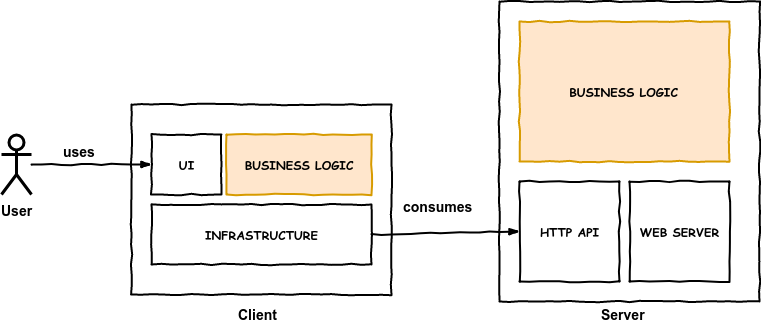
\includegraphics[width=450pt]
    {images/ui-dev-now.png}}
  \caption{A part of the business logic is hard coded into the client.}
  \label{fig:hardcoded}
\end{figure}

\subsection{Strategy}\label{strategy}
With this thesis we aim to identify types of complexity in UI and web development and suggest an approach to reduce them.
We want to minimize the manual work by leveraging linked data, the declarative concept of web components, the interaction model of task-based computing and by using hypermedia.

The expected results and artifacts consist of a proof-of-concept for a UI framework, n HTTP hypermedia vocabulary based on linked data, an interaction model influenced by task-based computing and the implementation of two use cases that showcase the UI framework. \\
Furthermore, we evaluate the UI framework in terms of its effect on software complexity. By reducing the complexity we aim to reduce the overall costs in UI and web development.

\subsection{Industrial partner}
The industrial partner of this thesis is Miko Nieminen Consulting. Miko Nieminen Consulting is interested in pushing open source efforts in linked data driven UI with complex user interaction. A future real-world use case is the generation of UIs for administrators.

\section{Background}\label{background}

This section discusses the problems with the process of developing UIs today. It also provides the theoretical backgroung by highlighting the main building blocks of the UI framework.

\subsection{Accidental and Essential Complexity}\label{history}

According to Turing Award winner Fred Brooks there are two types of complexity: accidental complexity and essential complexity. \citep{nosilverbullet}
In software engineering, \textbf{essential complexity} is complexity that comes from the domain problem that we want to solve. It is inherent to the problem that the customer cares about and its solution delivers business value. \textbf{Accidental complexity} is complexity that is caused by everything else. Compilers, distributed systems and databases are all examples for accidental complexity. In fact even programming languages and computers are often accidental complexity since they are not essential to the customer's problem.

This implies that accidental complexity could be eradicated in an ideal world. An example of such scenario is an executable specification: It comprises only business rules which are essential to the problem of the business, it doesn't contain any accidental complexity.

Ben Moseley and Peter Marks explore a general infrastructure to run specifications in their paper Out of the Tar Pit \citep{outoftarpit}.

Software engineering is itself an everlasting fight against accidental complexity. This is indeed the main goal of the UI Framework.

\subsection{Evolution of UI web development}\label{history}

In the early days of the Internet, websites were mostly \textbf{static files} accessible under certain URLs. Those files were often created manually or generated by using WYSIWYG editors. The served files were mostly styles (CSS), static assets and markup that the browsers had to render.

\textbf{Dynamically generated} content became popular with the rise of PHP. Websites were now able to show different things to each user based on previous interactions. The files that were served to the browsers were still the same static files. The markup was not hard coded anymore but dynamically rendered on the server upon user request.
\\ Developers had to work with templating languages to implement UIs that received that usually from the same server.

Websites became \textbf{truly interactive} with the introduction of AJAX. AJAX allowed the browser to asynchronously communicate with the server while the user was interacting with the website. Google was able to give search suggestions in real-time while the user was typing the search term. Websites were still rendered on the server but the served files additionally contained JavaScript that was run by the browser.
\\ UI development involved working with templating languages, styling and a small amount of programming.

The amount of interactive elements on websites and their \textbf{complexity increased}. What was once a text input field with real-time suggestions is now a full-text search interface with complex filtering and sorting options. The standardization of browser APIs was in the early stages and developers had to spend effort to create a consistent user experience across various browsers.
\\ Tools like jQuery emerged that provided a single interface for multiple browsers. The websites were still dynamically rendered on the server and just enriched in the browser by running JavaScript.

The first applications appeared providing a user experience in the browser similar to the one of fat desktop applications. The files that the server sent to the browser were mostly JavaScript. The browser ran that JavaScript application to render the website and to react on user input. It communicated with the server using AJAX and the website was not rendered on the server anymore. Instead a single website was served on which the whole application lifecycle took place. \textbf{Single page applications} (SPA) were born.
\par Development of UIs has drastically changed because the UI was part of an application that had its own lifecycle. Development of the server and the client application often took place separated. The HTTP API often played the role of an informal contract between client and server.

\subsection{Document Object Model}\label{documentobjectmodel}

The Document Object Model (DOM) is a programming API for HTML and XML documents. It defines the logical structure of documents and the way a document is accessed and manipulated. \citep{dom} The DOM exposes an \textbf{imperative} API to the developer.

We consider following HTML document:

\lstset{language=XML}
\begin{lstlisting}[caption=HTML document of a table, label=htmloftable]
<table>
  <rows>
    <tr>
      <td>Walter</td>
      <td>White</td>
    </tr>
    <tr>
      <td>Saul</td>
      <td>Goodman</td>
    </tr>
  </rows>
</table>
\end{lstlisting}

The DOM representation of that table looks as follows:

\begin{figure}[!htb]
  \center{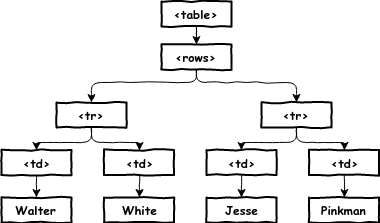
\includegraphics[width=250]
    {images/dom.png}}
  \caption{\label{fig:my-label} The DOM is a tree data structure representing an HTML document.}
\end{figure}

This process of creating the DOM given a document with markup takes place in the browser during \textbf{rendering}.

\subsection{UI web development today}\label{uidevelopmenttoday}

To this day a lot of UIs are developed that way. Some parts are increasingly rendered on the server again, mainly for performance and search engine optimization. It is common to have a \textbf{frontend} team working on the client and a \textbf{backend} team working on the server. The frontend team makes sense of the data that comes from the server either manually or in the best case using some form of HTTP API documentation.
\\ There are efforts like Swagger or OpenAPI to formalize and standardize documentation of HTTP APIs. Often documentation can be generated to a certain extent, so the overhead to keep the up-to-date is small. Documentation helps \textbf{humans} (frontend team) to understand the data and to develop a client that consumes the documented API in an efficient and effective way.
\\ Nevertheless, data coming from the server has to be understood by human frontend developers. That interpretation of the meaning of the incoming data is hard coded into the client and the UI. This causes strong coupling of the client to the data and therefore to the server. The client can not be re-used in some other \textbf{context}.

\subsubsection{Lack of context}\label{datahumanmachine}

Picture a scenario in everyday life where two good friends meet. One of them says: \textit{Have you heard about Frank? He recently got married.} Chances are high the other one knows multiple people named \textbf{Frank}. Being a human, he is able to map the name \textbf{Frank} to the person the other one is referring to. He is able to do so, because that conversation has an implicit context. That context is the intersection of the sets of people \textbf{both know}.
\par Exactly the same thing happens frequently in software development, especially in data exchange. A frontend developer looks at either all HTTP routes of an API or glances over the documentation. Sometimes he is able to \textbf{infer} the domain model because of his personal experiences as a human. If that developer is not familiar with the domain at all, maybe because the domain is niche, he has trouble understanding the data coming from the server. He perceives development to be difficult and he is not able to put the data being exchanged into a \textbf{context}.
\par What makes the life of a human developer hard, poses an insurmountable obstacle to a machine. A machine doesn't have dozens of years of life experience to draw from when trying to understand data.\footnote{Here we talk about machines in the sense of contemporary information systems. Systems that are able to learn are deliberately ignored as they haven't been proven to be useful in this context.} The machine has to be fed a context together with the data it should understand. In traditional web UI development that context is hard coded into the client and the UI. The author believes that the majority of work done in UI development could be eliminated by \textbf{exchanging data that has meaning attached to it}.

\subsection{Web components}\label{webcomponents}

In recent years an approach to rendering UIs became popular which we will call \textbf{component-based} rendering. This paragraph analyzes the reason why this approach to UI development gained popularity.

\subsubsection{React}

In 2013 Facebook released a library called React, which today is still one of the main tools for web development. It was one of the first libraries to encourage the usage of \textbf{web components}. Due to its widespread adoption in web development it caused a paradigm shift.

React encourages the thinking of UIs as a composition of \textbf{web components}. The UI developer doesn't touch the DOM manually and merely provides data to React. This is a declarative approach where the developer states \textbf{what} not \textbf{how} the UI should be rendered. \\
Most importantly, React models the problem of UI rendering as function application. This insight leads to small re-usable components which has various benefits.


\begin{figure}[!htb]
  \center{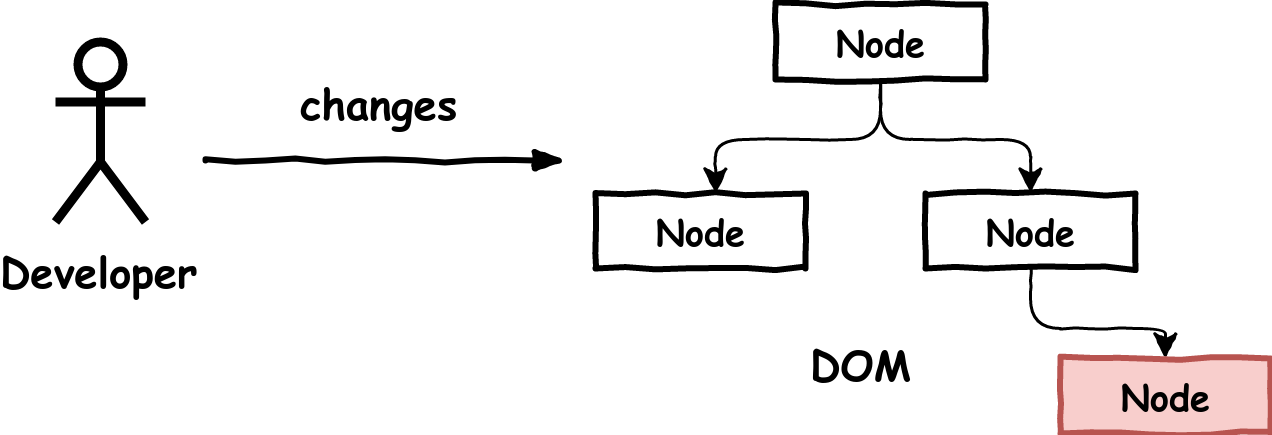
\includegraphics[width=250]
    {images/ui-imperative.png}}
  \caption{\label{fig:my-label} Imperative development: Developer works directly with DOM.}
\end{figure}

\begin{figure}[!htb]
  \center{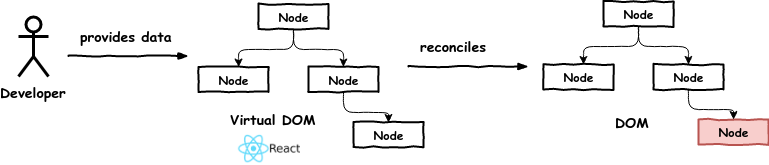
\includegraphics[width=380]
    {images/ui-declarative.png}}
  \caption{\label{fig:my-label} Declarative development: Developer provides data and React takes care of the DOM.}
\end{figure}

The markup output of a component depends only on its data input. This allows to understand the change in the output when changing the input, the component is \textbf{easy to reason about}. It can be \textbf{tested easily in isolation} because there are no other dependencies than the data input. Analogous to function composition, such web components can be \textbf{composed} to larger UIs. Because web components are designed to be self-contained, they have high cohesion which makes them usable in multiple contexts. That means a good code \textbf{reuse can be achieved}.

\subsubsection{Templates vs. Component}

TODO: Quote Riotjs

\subsection{Richardson Maturity Model and HATEOAS}

TODO

\subsection{Linked data}\label{linkeddata}

Linked data is a way of creating a web of machine interpretable data across different domains, systems and organizations. A person or a machine should be able to explore data by simply following links. In essence, the same expectations apply to make that web of data grow as to linked HTML documents: \citep{linkedatafourrules}

\begin{enumerate}
  \item Use URIs as names for things
  \item Use HTTP URIs so that people can look up those names.
  \item When someone looks up a URI, provide useful information, using the standards (RDF*, SPARQL)
  \item Include links to other URIs, so that they can discover more things.
\end{enumerate}

A machine looking at a piece of linked data follows the links and is able to unambiguously understand the data. This is equivalent of traversing a graph since linked data is effectively a giant graph. There are multiple serialization formats in the family of specifications called Resource Description Framework (RDF) \citep{rdfspecification}.

An RDF file describing a Smith family could live at \lstinline{http://example.org/smith} and have following content:

\lstset{language=XML}
\begin{lstlisting}[caption= Simple example of a person as RDF, label=rdfexample]
<rdf:Description about="#albert"
 <fam:child rdf:Resource="#brian">
  <fam:child rdf:Resource="#carol">
  </rdf:Description>
\end{lstlisting}

Information about the grandparent Albert can be obtained by loading the data at \\ \lstinline{http://example.org/smith#albert}. Albert's child Brian can be accessed at \\  \lstinline{http://example.org/smith#brian} and Brian's child Carol at \lstinline{http://example.org/smith#carol}.

\subsection{JSON-LD}\label{jsonld}

TODO mention users of JSON-LD: https://github.com/json-ld/json-ld.org/wiki/Users-of-JSON-LD

In web development the main format for data exchange now is JSON \citep{jsonformat}. It is easy to parse and to generate and many languages provide first-class support for it.

However, JSON is difficult to integrate from different sources as the data may contain keys that conflict with other data sources. JSON has no built-in support for hyperlinks, which are a fundamental building block on the Web \citep{jsonldbasicconcepts}.

Consider following JSON snippet:

\lstset{language=JSON}
\begin{lstlisting}[caption=Data of a person in the JSON format, label=jsonexample]
{
  "name": "Manu Sporny",
  "homepage": "http://manu.sporny.org/",
  "image": "http://manu.sporny.org/images/manu.png"
}
\end{lstlisting}

It's obvious to humans that the data is about a person whose name is \textit{Manu Sporny} and that the homepage property contains the URL of that person's homepage. A machine doesn't have such an intuitive understanding and sometimes, even for humans, it is difficult to resolve ambiguities in such representations. This problem can be solved by using unambiguous identifiers to denote the different concepts instead of tokens such as \textbf{name} or \textbf{homepage} \citep{jsonldbasicconcepts}.

JSON-LD is a serialization format for linked data and is based on JSON-LD. By using the popular schema.org vocabulary the example \ref{jsonexample} can be written as follows:

\lstset{language=JSON}
\begin{lstlisting}[caption=Data of a person in the JSON-LD format, label=jsonldexample]
{
  "http://schema.org/name": "Manu Sporny",
  "http://schema.org/url": {
    "@id": "http://manu.sporny.org/"
  },
  "http://schema.org/image": {
    "@id": "http://manu.sporny.org/images/manu.png"
  }
}
\end{lstlisting}

This can be understood by any machine without providing additional information. The key \lstinline{http://schema.org/name} can be looked up to determine the meaning of the value \lstinline{Manu Sporny}. JSON-LD supports the concept of a \textbf{context}.

The context is meta data that has to be provided together with the data. This makes it possible for a machine to attach meaning to it. Thanks to the context it is not required to have the keys as absolute URIs anymore. The data can be compacted and written as follows:

\lstset{language=JSON}
\begin{lstlisting}[caption=Compacted data of a person, label=jsonldcompacted]
{
  "@context": "http://schema.org",
  "name": "Manu Sporny",
  "url": "http://manu.sporny.org/",
  "image": "http://manu.sporny.org/images/manu.png"
}
\end{lstlisting}

With the small addition of the reserved keyword \lstinline{@context} readability of JSON was restored while allowing machines to understand the data. JSON-LD is 100\% compatible with JSON and therefore benefits of the vast amount of JSON tooling available.

There are a few operations that can be executed on JSON-LD. Following are the three most important ones for this thesis:

\subsubsection{Framing}\label{jsonldframing}

Framing is an operation that re-shapes the data. Input of the framing operation is data and a \textbf{frame}. The frame determines the new shape of the data.

Consider following data of a library. The data is in the form of a normalized graph. The \lstinline{contains} relation represents edges between nodes, the items in the \lstinline{@graph} list are the graph nodes.

\lstset{language=JSON}
\begin{lstlisting}[caption=Data of a library as normalized graph]
{
  "@context": {
    "@vocab": "http://example.org/",
    "contains": {"@type": "@id"}
  },
  "@graph": [{
    "@id": "http://example.org/library",
    "@type": "Library",
    "contains": "http://example.org/library/the-republic"
  }, {
    "@id": "http://example.org/library/the-republic",
    "@type": "Book",
    "creator": "Plato",
    "title": "The Republic",
    "contains": "http://example.org/library/the-republic#introduction"
  }, {
    "@id": "http://example.org/library/the-republic#introduction",
    "@type": "Chapter",
    "description": "An introductory chapter on The Republic.",
    "title": "The Introduction"
  }]
}
\end{lstlisting}

Following frame determines the shape of the frame data:

\lstset{language=JSON}
\begin{lstlisting}[caption=Frame for the framing operation]
{
  "@context": {
    "@version": 1.1,
    "@vocab": "http://example.org/"
  },
  "@type": "Library",
  "contains": {
    "@type": "Book",
    "contains": {
      "@type": "Chapter"
    }
  }
}
\end{lstlisting}

The result of the framing operation is a tree:

\lstset{language=JSON}
\begin{lstlisting}[caption=Framed data of a library]
{
  "@context": {
    "@version": 1.1,
    "@vocab": "http://example.org/"
  },
  "@id": "http://example.org/library",
  "@type": "Library",
  "contains": {
    "@id": "http://example.org/library/the-republic",
    "@type": "Book",
    "contains": {
      "@id": "http://example.org/library/the-republic#introduction",
      "@type": "Chapter",
      "description": "An introductory chapter on The Republic.",
      "title": "The Introduction"
    },
    "creator": "Plato",
    "title": "The Republic"
  }
}
\end{lstlisting}

\subsubsection{Compacting}\label{jsonldcompacting}

Compacting describes the operation of reducing verbosity in the JSON-LD data. Compacted data is meant to be read and understood by human developers. This is achieved by pulling out the context and explicitely define it using the \lstinline{@context} keyword.

Consider following input:

\lstset{language=JSON}
\begin{lstlisting}[caption=Verbose data of a person]
{
  "http://schema.org/name": "Manu Sporny",
  "http://schema.org/url": {
    "@id": "http://manu.sporny.org/"
  },
  "http://schema.org/image": {
    "@id": "http://manu.sporny.org/images/manu.png"
  }
}
\end{lstlisting}

This data can be compacted by pulling out the \lstinline{@context}:

\lstset{language=JSON}
\begin{lstlisting}[caption=Compacted and easy-to-read data of a person]
{
  "@context": "http://schema.org",
  "name": "Manu Sporny",
  "url": "http://manu.sporny.org/",
  "image": "http://manu.sporny.org/images/manu.png"
}
\end{lstlisting}

\subsubsection{Expanding}\label{jsonldextending}

Expanded data serves the opposite goal of compacting data. While compacted data is easy to read for humans, extended data is easy to process for machines.

Expanding the following compacted data

\lstset{language=JSON}
\begin{lstlisting}[caption=Compacted and easy-to-read data of a person]
{
  "@context": "http://schema.org",
  "name": "Manu Sporny",
  "url": "http://manu.sporny.org/",
  "image": "http://manu.sporny.org/images/manu.png"
}
\end{lstlisting}

results in following expanded data:

\lstset{language=JSON}
\begin{lstlisting}[caption=Expanded data of a person that is easy to process for machines]
[
  {
    "http://schema.org/image": [
      {
        "@id": "http://manu.sporny.org/images/manu.png"
      }
    ],
    "http://schema.org/name": [
      {
        "@value": "Manu Sporny"
      }
    ],
    "http://schema.org/url": [
      {
        "@id": "http://manu.sporny.org/"
      }
    ]
  }
]
\end{lstlisting}

\subsection{Vocabulary}

JSON-LD is essentially a linked data serialization format that plays well with JSON tooling. Creating linked data means creating a vocabulary that other might use by linking to it. A lot of vocabularies those exist and two of them are particularly interesting for this thesis.

\subsubsection{Schema.org}

\url{Schema.org} is a collaborative, community activity with a mission to create, maintain, and promote schemas for structured data on the Internet, on web pages, in email messages, and beyond \citep{welcomeschemaorg}. Companies like Google, Microsoft, Pinterest and Yandex are using it in their tools and products.

Their main goal is to provide a shared vocabulary that web developers can refer to. It is often used in the context of search engine optimization by helping crawlers understand websites.

Schema.org is a hierarchy of \lstinline{Things} that have an implicit \textbf{is a} relationship. This is similar to sub typing through inheritance in many object-oriented programming languages. Following is a small subset of the Schema.org hierarchy:

\begin{figure}[!htb]
  \center{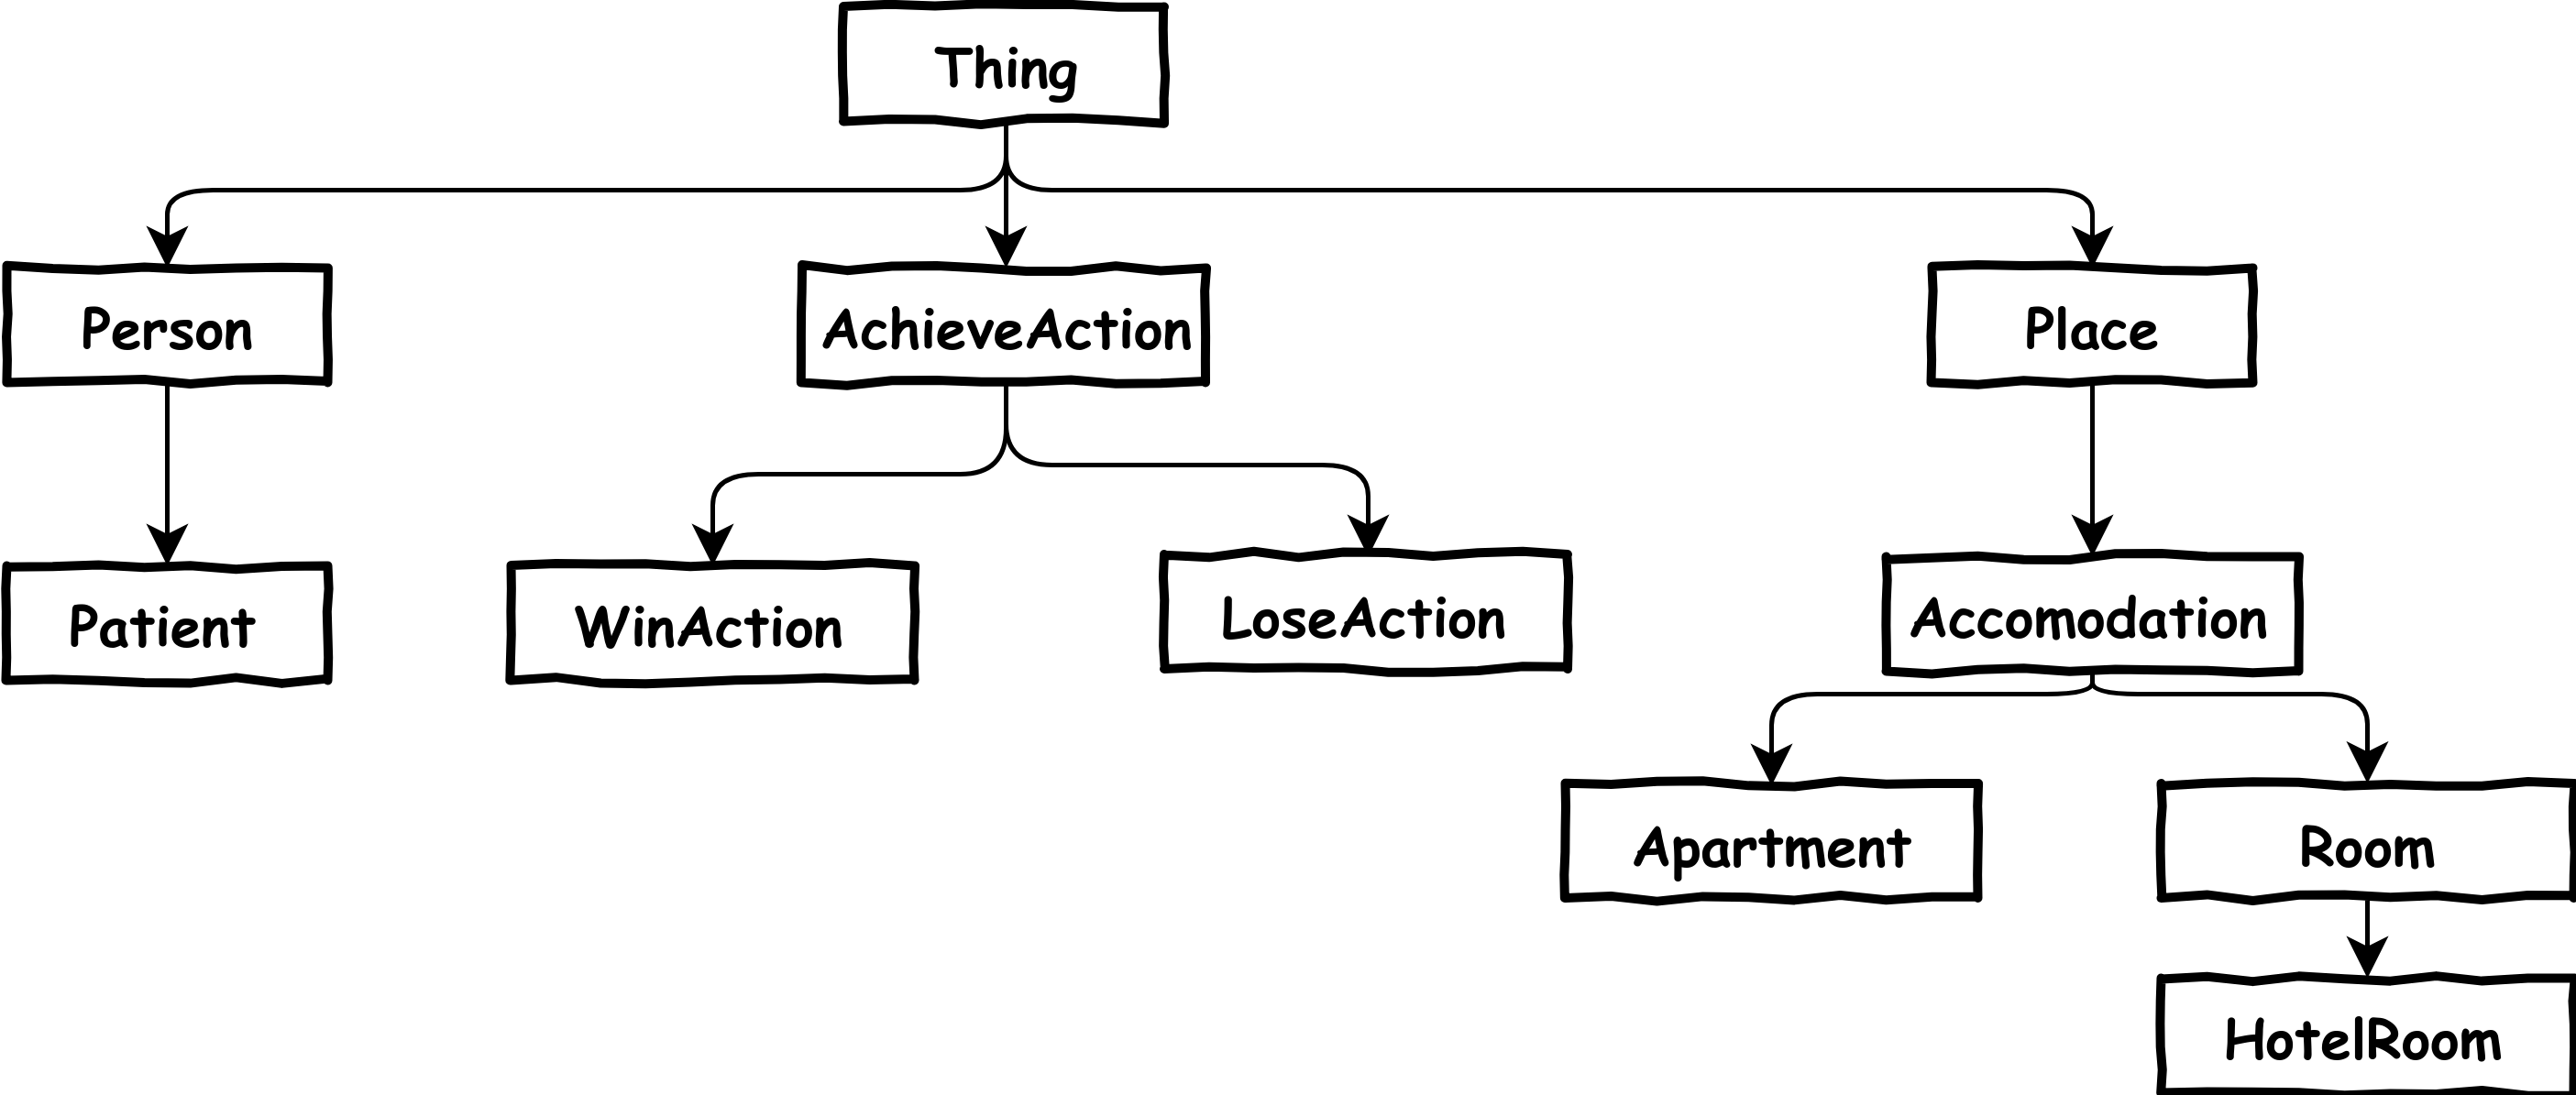
\includegraphics[width=300]
    {images/schemaorg.png}}
  \caption{\label{fig:schemaorg} Subset of the Schema.org ontology where child-parent relation describes an \textit{is a} relationship.}
\end{figure}

The advantage of using such a vocabulary becomes obvious when looking at an example.The type \lstinline{Person} has a property \lstinline{address}. \lstinline{Address} can be of type \lstinline{http://schema.org/Text} or \lstinline{http://schema.org/PostalAddress}.

\lstset{language=JSON}
\begin{lstlisting}[caption=A person with an address of type Text]
{
  "@context": "http://schema.org",
  "givenName": "Walter",
  "familyName": "White",
  "address": "3828 Piermont Dr NE Albuquerque, NM 87111, USA"
}
\end{lstlisting}

A machine receiving that data knows that this is a person and understands his name, but it can not understand his address. There is additional context needed that describes the schema used in the \lstinline{address} property.

The data of the same person where the address is of type \lstinline{http://schema.org/PostalAddress} can be processed unambiguously by any machine that understands linked data.

\lstset{language=JSON}
\begin{lstlisting}[caption=A person with an address of type PostalAddress]
{
  "@context": "http://schema.org",
  "givenName": "Walter",
  "familyName": "White",
  "address": {
    "@type": "PostalAddress",
    "addressLocality": "Albuquerque",
    "addressRegion": "NM",
    "postalCode": "87111",
    "streetAddress": "3828 Piermont Dr NE Albuquerque"
  },
}
\end{lstlisting}

The \lstinline{streetAddress} is still stringly typed. A system running at a package distribution center could route packages correctly to some local distribution center or postal office by looking at \lstinline{addressRegion} and \lstinline{addressLocality}.

\subsubsection{Hydra}

\href{http://www.hydra-cg.com/}{Hydra} is a lightweight vocabulary to create hypermedia-driven Web APIs. By specifying a number of concepts commonly used in Web APIs it enables the creation of generic API clients.\citep{hydasprecs}

\subsection{Landscape of solutions and tools}

\subsubsection{GraphQL}
\subsubsection{Rails with ActiveAdmin}
\subsubsection{Hyperfiddle}
\subsubsection{Fulcro}

\section{Analysis}
\subsection{Risk analysis}\label{sec:riskanalysis}

\paragraph{Methodology}
We identify risks that could affect the implementation of the UI framework and the use cases. Each risk has a probability of occurrence as shown in table \ref{tab:probability} and a severity as explained in table \ref{tab:severity}. Multiplication of both scores yields the risk factor. We list all risks sorted descending by their risk factor in table \ref{tab:riskanalysis}. A risk factor greater or equal \textbf{8} indicates a risk that is likely to cause substantial project damage. \\
Furthermore, decisions that are made in section \ref{sec:proofofconcept} are based on this sorted list of risks.

\begin{table}[!htb]
  \begin{center}
    \begin{tabular}{|l|l|l|}
      \hline
      \textbf{Probability} & \textbf{Score} & \textbf{Description} \\
      \hline
      0 <= p <= 0.25 & 1 & The probability of occurrence of this risk is minimal. \\
      \hline
      0.25 < p <= 0.5 & 2 & The risk might occur with a low probability. \\
      \hline
      0.5 < p <= 0.75 & 3 & There is a significant chance for the risk to occur. \\
      \hline
      0.75 < p <= 1 & 4 & The probability of occurrence of this risk is high. \\
      \hline
    \end{tabular}
    \caption{The probability of occurrence is mapped to a score which is used in the risk analysis.}
    \label{tab:probability}
  \end{center}
\end{table}

\begin{table}[!htb]
  \begin{center}
    \begin{tabular}{|l|l|l|}
      \hline
      \textbf{Severity} & \textbf{Score} & \textbf{Project Damage} \\
      \hline
      insignificant & 1 & \begin{tabular}[x]{@{}l@{}}It is possible to implement the UI framework and the use cases \\ but the results might be poor.\end{tabular} \\
      \hline
      moderate & 2 & \begin{tabular}[x]{@{}l@{}}It is possible to implement the UI framework and the use cases \\ but the results might be unusable.\end{tabular} \\
      \hline
      high & 3 & \begin{tabular}[x]{@{}l@{}}It is possible to implement the UI framework and the use cases. \\ That approach to UI development is less efficient and more \\ costly than UI development without the UI framework.\end{tabular} \\
      \hline
      fatal & 4 & \begin{tabular}[x]{@{}l@{}}It is not possible to implement the UI framework and the use cases.\end{tabular} \\
      \hline
    \end{tabular}
    \caption{The level of severity is mapped to a score which is used in the risk analysis.}
    \label{tab:severity}
  \end{center}
\end{table}

\begin{table}[!htb]
  \begin{center}
    \begin{tabular}{|l|l|}
      \hline
      \textbf{ID} & R1 \\
      \hline
      \textbf{Title} & Incomplete HATEOAS specification \\
      \hline
      \textbf{Probability of occurrence} & 2 \\
      \hline
      \textbf{Severity} & 4 \\
      \hline
      \textbf{Risk Factor} & 8 \\
      \hline
      \textbf{Description} & \begin{tabular}[x]{@{}l@{}}The HATEOAS specification in use is either an early draft or it \\ has been abandoned. In the worst case, the specification superficially \\ appears to be complete while not providing crucial features that \\ are needed by the use cases. Parts of it have to be written during the \\ thesis work.\end{tabular} \\
      \hline
    \end{tabular}
    \caption{Source of risk R1.}
  \end{center}
\end{table}

\begin{table}[!htb]
  \begin{center}
    \begin{tabular}{|l|l|}
      \hline
      \textbf{ID} & R2 \\
      \hline
      \textbf{Title} & Unstable HATEOAS specification and tooling\\
      \hline
      \textbf{Probability of occurrence} & 3 \\
      \hline
      \textbf{Severity} & 1 \\
      \hline
      \textbf{Risk Factor} & 3 \\
      \hline
      \textbf{Description} & \begin{tabular}[x]{@{}l@{}}The HATEOAS specification in use and reference implementations \\ are under development and parts are rewritten frequently. For the \\ thesis work a version has to be pinpointed.\end{tabular} \\
      \hline
    \end{tabular}
    \caption{Source of risk R2.}
  \end{center}
\end{table}

\clearpage

\begin{table}[!htb]
  \begin{center}
    \begin{tabular}{|l|l|}
      \hline
      \textbf{ID} & R3 \\
      \hline
      \textbf{Title} & Lack of HATEOAS tooling \\
      \hline
      \textbf{Probability of occurrence} & 2 \\
      \hline
      \textbf{Severity} & 2 \\
      \hline
      \textbf{Risk Factor} & 4 \\
      \hline
      \textbf{Description} & \begin{tabular}[x]{@{}l@{}}The HATEOAS specification in use has no reference implementation, \\ little working examples and no tools for generating and consuming \\ HATEOAS APIs. All tools have to be written from scratch.\end{tabular} \\
      \hline
    \end{tabular}
    \caption{Source of risk R3.}
  \end{center}
\end{table}

\begin{table}[!htb]
  \begin{center}
    \begin{tabular}{|l|l|}
      \hline
      \textbf{ID} & R4 \\
      \hline
      \textbf{Title} & Lack of JSON-LD tooling \\
      \hline
      \textbf{Probability of occurrence} & 1 \\
      \hline
      \textbf{Severity} & 3 \\
      \hline
      \textbf{Risk Factor} & 3 \\
      \hline
      \textbf{Description} & \begin{tabular}[x]{@{}l@{}}There are no tools that implement the JSON-LD operations \\ discussed in section \ref{jsonld}. The used languages and frameworks don't \\ support JSON as first-class citizen \footnote{A language treats JSON as first-class citizen if it supports it natively.}. All tools have to be written \\ from scratch.\end{tabular} \\
      \hline
    \end{tabular}
    \caption{Source of risk R4.}
  \end{center}
\end{table}

\begin{table}[!htb]
  \begin{center}
    \begin{tabular}{|l|l|}
      \hline
      \textbf{ID} & R5 \\
      \hline
      \textbf{Title} & Lack of design language implementations \\
      \hline
      \textbf{Probability of occurrence} & 1 \\
      \hline
      \textbf{Severity} & 4 \\
      \hline
      \textbf{Risk Factor} & 4 \\
      \hline
      \textbf{Description} & \begin{tabular}[x]{@{}l@{}}The UI framework provides usable UIs out of the box. These  \\ are created by using a design language implementation which \\ takes care of portability across browsers. The implementation provides \\ the authors with best practices in UI design and layout. In case \\ there is a lack of design language implementations, one has to \\ be written from scratch.\end{tabular} \\
      \hline
    \end{tabular}
    \caption{Source of risk R5.}
  \end{center}
\end{table}

\clearpage

\begin{table}[!htb]
  \begin{center}
    \begin{tabular}{|l|l|}
      \hline
      \textbf{ID} & R6 \\
      \hline
      \textbf{Title} & Linked data-driven UIs are slow \\
      \hline
      \textbf{Probability of occurrence} & 3 \\
      \hline
      \textbf{Severity} & 2 \\
      \hline
      \textbf{Risk Factor} & 6 \\
      \hline
      \textbf{Description} & \begin{tabular}[x]{@{}l@{}}JSON-LD operations as discussed in section \ref{jsonld} require multiple \\ requests per user request. This adds some overhead to \\ the client-server communication which can decrease performance. \\ If those additional requests can not be mitigated by caching, the \\ overhead might affect the \gls{ux}. \end{tabular} \\
      \hline
    \end{tabular}
    \caption{Source of risk R6.}
  \end{center}
\end{table}

\begin{table}[!htb]
  \begin{center}
    \begin{tabular}{|l|l|l|}
      \hline
      \textbf{ID} & \textbf{Risk Factor} & \textbf{Title} \\
      \hline
      \rowcolor{yellow}
      R1 & 8 & Incomplete HATEOAS specification \\
      \hline
      R6 & 6 & Linked data-driven UIs are slow \\
      \hline
      R5 & 4 & Lack of design language implementations \\
      \hline
      R3 & 4 & Lack of HATEOAS tooling \\
      \hline
      R2 & 3 & Unstable HATEOAS specification and tooling \\
      \hline
      R4 & 3 & Lack of JSON-LD tooling \\
      \hline
    \end{tabular}
    \caption{The result of the risk analysis shows the list of all risks sorted descending by their total risk factor. R1 has a large impact on the success of the project.}
    \label{tab:riskanalysis}
  \end{center}
\end{table}

\subsection{Conceptual analysis of user interfaces}
For a system to be useful, it has to interact with its environment. These interactions happen through multiple types of interfaces, which are used by either other systems or human users.
Interfaces for human users share fundamental properties. By observing their usage we can analyze the main characteristics. A typical scenario of UI usage is browsing a website. At all times, while using the website, the user either reads or clicks.

The UI has to present information that the user \textbf{reads} and it has to provide means for \textbf{interaction}. In terms of operations on data, this is equivalent to \textbf{querying} and \textbf{mutating or commanding}.

\begin{enumerate}
  \item Query: The user is able to retrieve information by looking at the UI
  \item Interaction: The user is able to interact with the UI
\end{enumerate}

These two fundamental properties of UIs are driving the definition and implementation of the two use cases.

\subsection{Analysis of HATEOAS API specifications}\label{sec:analysishateoas}
The goal is to chose a specification among existing HATEOAS API specifications. The real-world uses cases will implement HTTP APIs that conform to this specification \footnote{The actual implementation of those APIs is not the concern of this thesis. The focus is on the choice and evaluation of a HATEOAS specification.}. The client that consumes that API is merely a \gls{console}. This implies the client doesn't contain any knowledge about the API implementation. \\
We enumerate the requirements for a HATEOAS specification from the point of view of a consumer.

\paragraph{Self documenting}
The API should provide its own documentation so the consumer is not reliant on additional tools to consume documentation. The API should document itself which requires a mechanism to attach meta data to the response payload.

\paragraph{Discoverability}
The consumer should be able to autonomously discover the data model of an API by autonomously building and invoking requests.

\paragraph{Actions and Operations}
The API should provide a description on how to interact with it. It publishes the information that is needed by the consumer to build and invoke requests.

\paragraph{Uses linked data}
Based on the discussion in section \ref{linkeddata} about the benefits of \gls{linkeddata}, we explore \gls{linkeddata} as the key component to efficient UI development. The combination with web component based rendering discussed in section \ref{webcomponents} allows UI developers to think in terms of components and data.

\subsubsection{Hydra}
It is remarkable that at the time of writing this thesis, only one HATEOAS specification exists that satisfies the requirements stated in section \ref{sec:analysishateoas}.

\textit{``\href{http://www.hydra-cg.com/}{Hydra} is a lightweight specification to create hypermedia-driven Web APIs. By specifying a number of concepts commonly used in Web APIs, it enables the creation of generic API clients \citep{hydraspecs}.''} At the time of writing, the Hydra specification exists as an unofficial draft.

Two benefits of APIs supporting hypermedia are \textbf{discoverability} and \textbf{self documentation}.

\paragraph{Discoverability} Discoverability is given by the RESTful nature of any hypermedia API. The API provides an entry point and each resource describes the means to fetch other resources using \gls{uri}s. The client is able to traverse the API by understanding the response and sending requests to the server - there is no external documentation needed to discover the API.

\paragraph{Self documentation}
Hydra documents itself by providing meta data along the payload. \\
It can use the same data model for generating built-in documentation and serving the API. These documentations are less likely to become out-of-date which reduces maintenance costs.

\paragraph{Collections, partial views and pagination}
In the world of Hydra, there are conceptually only \textit{things} and \textit{lists of things}. There is no list of list of things. \\
Hydra calls a list of things \textit{collection}, which can have things as members. There is the concept of a partial view. This gives the client the ability to fetch a subset of a collection. That partial view can be controlled by client initiated \gls{pagination}. The client provides a limit and an offset when requesting a collection in order to initiate \gls{pagination}.

\paragraph{Operations}
In order to interact with the server, a client has to know which operations the server supports. Hydra exposes all information necessary to build and invoke operations. This allows any client that understands Hydra to interact with it without any prior knowledge about the concrete API implementation. \\
This part is not fully specified yet at the time of writing. \footnote{We had to directly communicate with Hydra core members and reverse engineer tools in the Hydra ecosystem in order to understand how Hydra operations are supposed to work.}

\subsection{Analysis of design languages}
\textit{``A design language or design vocabulary is an overarching scheme or style that guides the design of a complement of products or architectural settings. Designers wishing to give their suite of products a unique but consistent look and feel define a design language for it, which can describe choices for design aspects such as materials, colour schemes, shapes, patterns, textures, or layouts. They then follow the scheme in the design of each object in the suite.''} \citep{designlanguage}

The benefit of using design languages is the consistent look and feel of UIs that are composed of a set of default components. Additionally, it frees UI developers from cumbersome work such as making sure that the UI is responsive and behaves well on various screen sizes. UI developers can communicate and think in a higher level of abstraction by omitting implementation details that are taken care of by the design language implementation. As an example, it allows for the mental model of small buttons horizontally next to each other while ignoring the implementation using CSS properties.

The major design languages are built on top of years of research in human-computer interaction. Evaluation of the theoretical foundation is not in the scope of this thesis. We aim to benefit off existing implementations and tools.

\subsubsection{Design language implementations}
The UI framework will consume React components provided by UI developers and it will use React for internal components as well. The only requirement for the design language implementation is the use of React.

\paragraph{Material Design}
Material Design was developed at Google in 2014. Initially it was used in Google's own mobile apps and in Android \footnote{Android is a mobile operating system developed by Google.}. In order to offer a consistent \gls{ux} across all products, Google uses it in web products as well.

The React implementation of Material Design is called Material UI \footnote{\url{https://material-ui.com/}}. It bottles up the \gls{ux} best practices and provides them in the form of React components. \\
By implementing a simple form with three text fields and a button, we conclude that Material UI is too heavyweight. It is not always obvious how to configure components - especially big ones. The main contribution of Material Design and Material UI are best practices in mobile \gls{ux}. This reaches beyond simple forms and visualization of lists. Material Design dictates the look and feel of the \gls{ux} holistically. \\
The UI framework requires a lower level design language implementation that doesn't make assumptions and doesn't state rules about larger components and \gls{ux}. These decisions have to be made by UI developers using the framework.

\paragraph{Semantic UI}
\textit{``Semantic empowers designers and developers by creating a shared vocabulary for UI.''} \citep{semanticui} This thesis explores the benefits of shared vocabularies by using linked data in HTTP APIs - the shared vocabulary of Semantic UI could be mapped to the shared vocabulary in the data. Semantic UI is not as widely adopted as Material Design. Its React implementation has a level of abstraction that fits generically rendering forms and navigation.

\begin{figure}[!htb]
  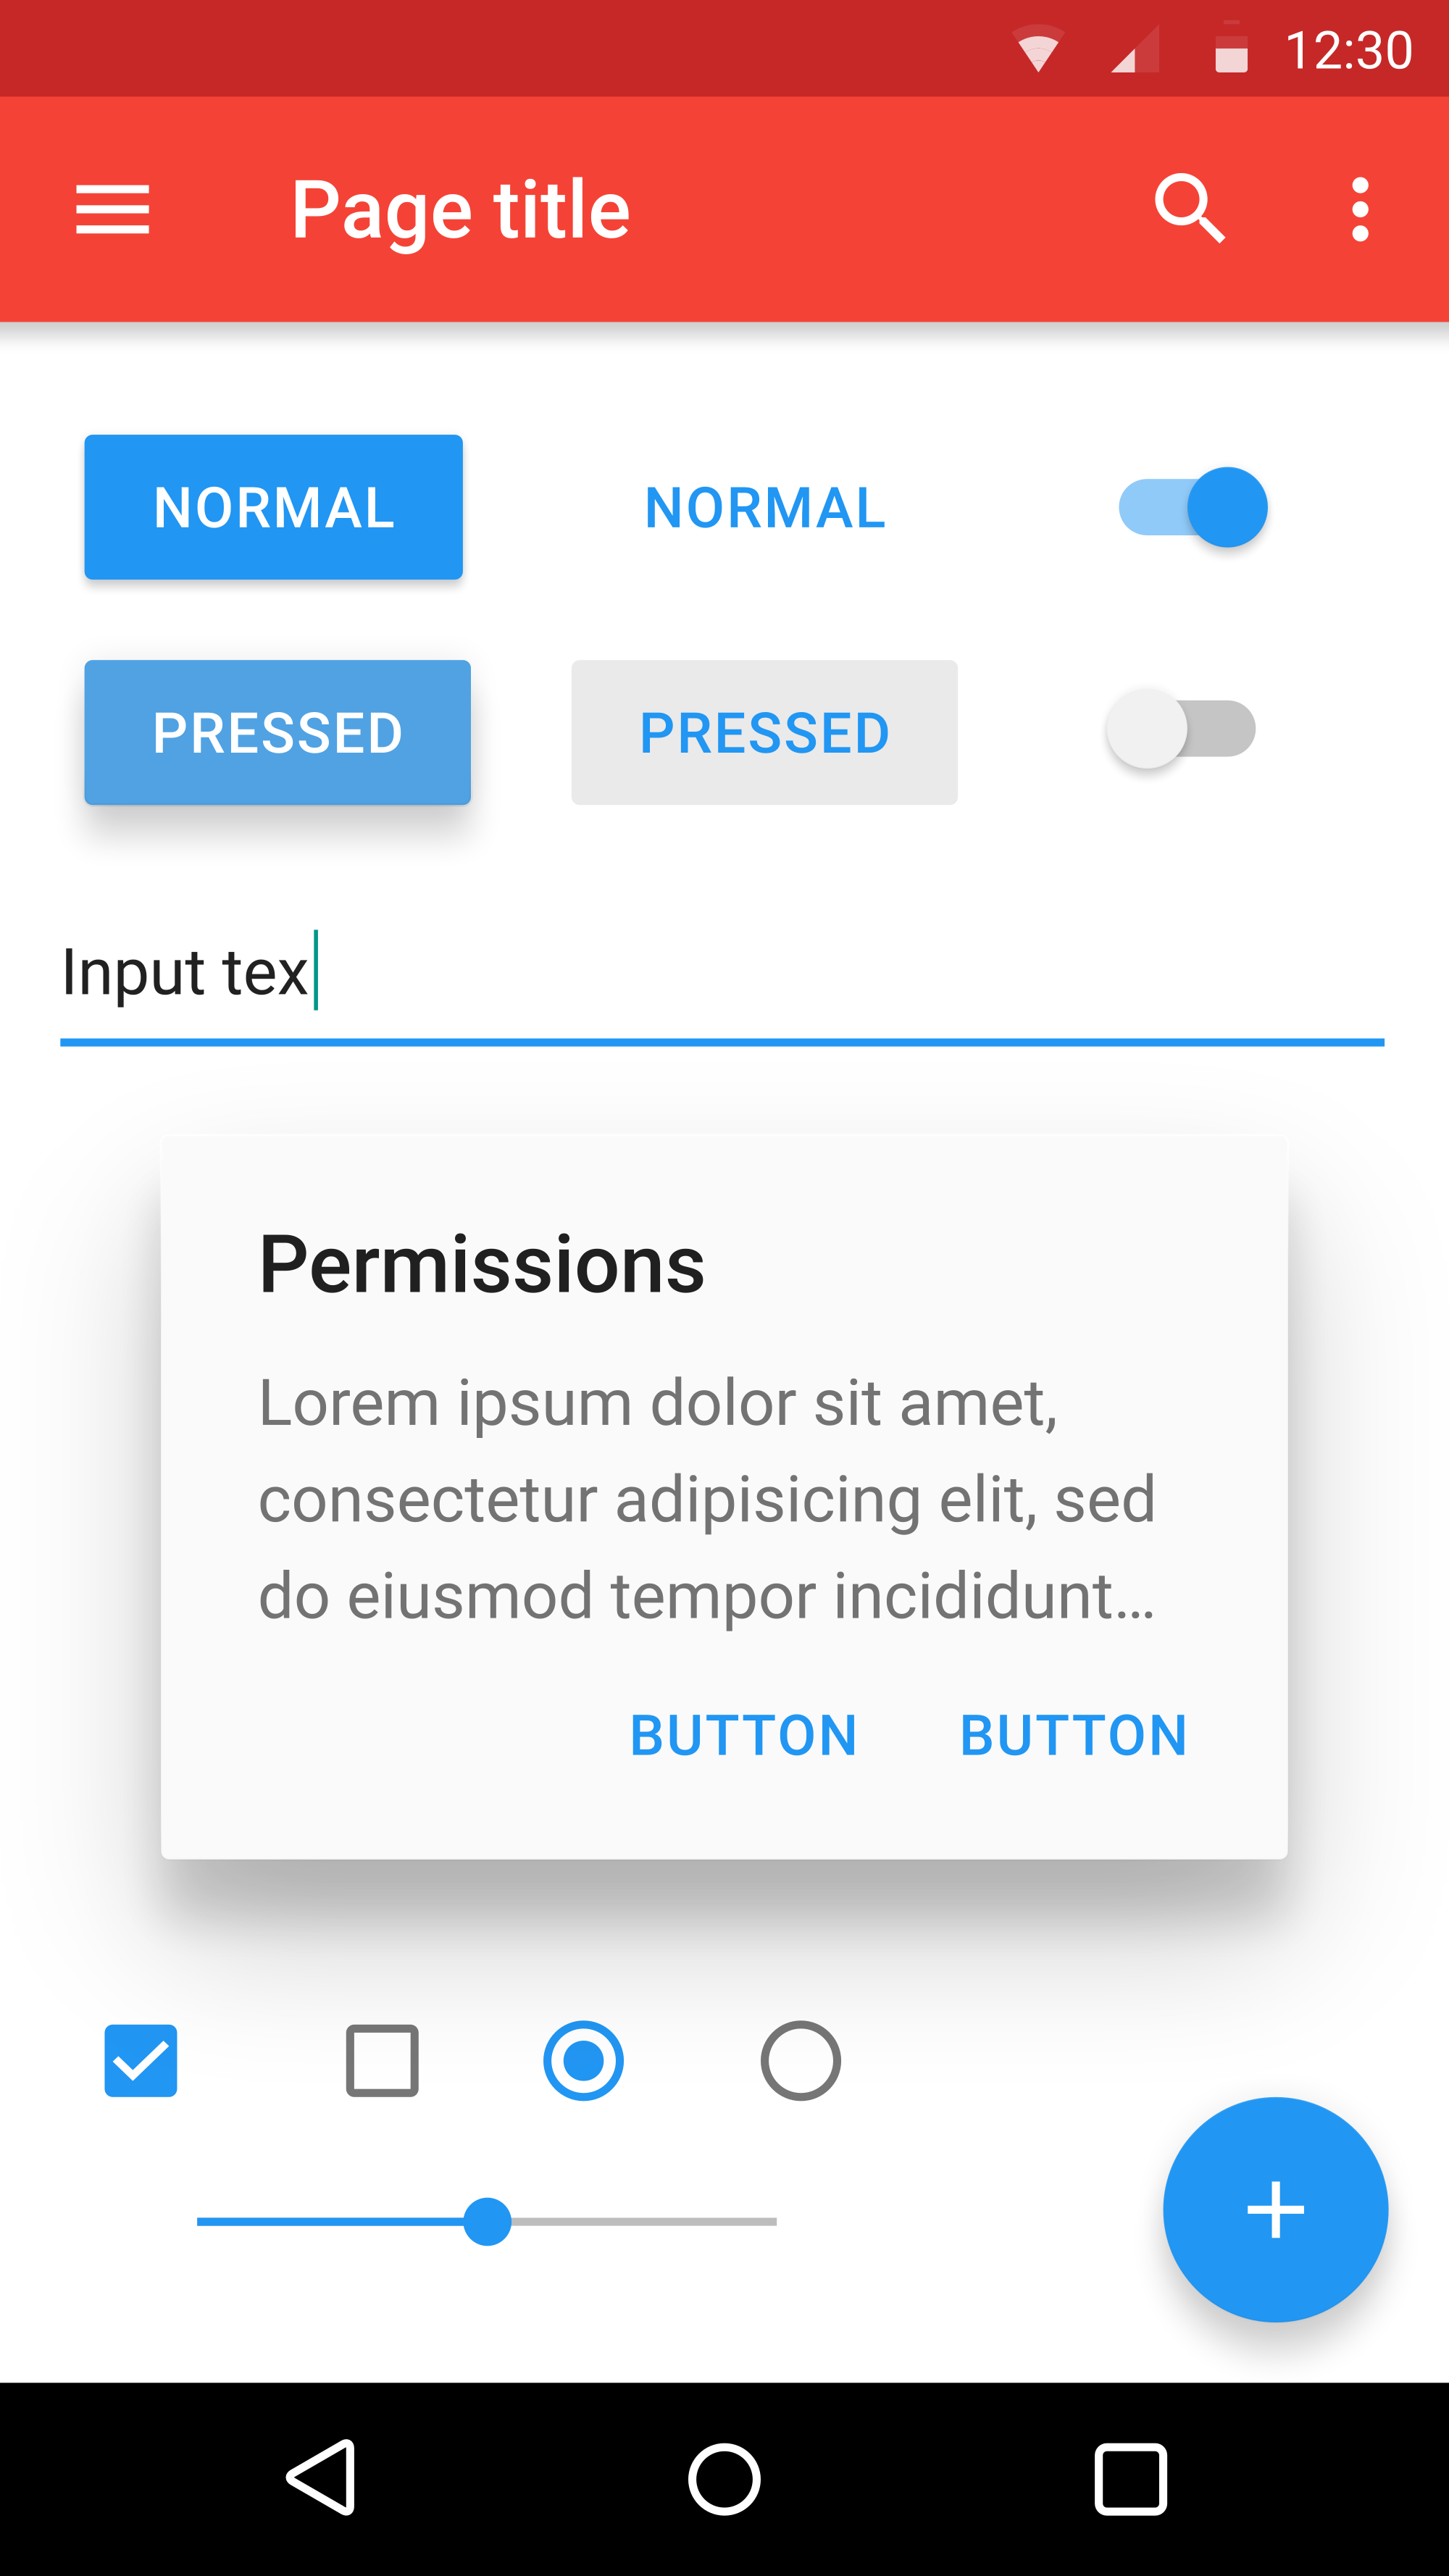
\includegraphics[width=150pt]
    {images/materialdesign.png}
  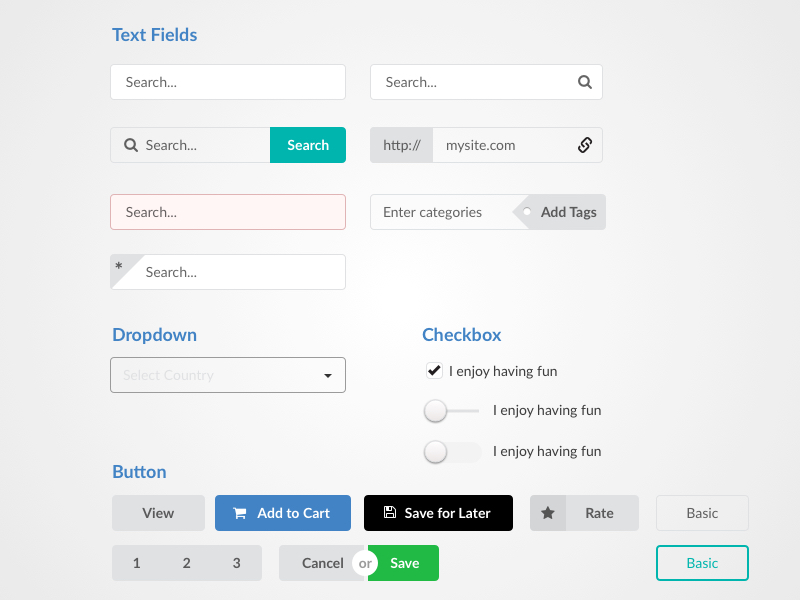
\includegraphics[width=320pt]
    {images/semanticui.jpg}
  \caption{Material Design on a mobile device (left) and Semantic UI components (right). \\ (Source: https://wikipedia.org, https://www.sketchappsources.com/)}
\end{figure}

We pick Semantic UI and its React implementation.

\section{Proof of concept}\label{sec:proofofconcept}
The main contribution of this thesis is the theoretical foundation and development of a new approach to UI development that reduces development costs.

\subsection{Methodology}
This sections describe the methodological approach to achieve the items listed in the paragraph \ref{sec:scope}.

\subsubsection{Steps}
This section explains the methods of this analysis.

\paragraph{Definition of major design goals}
Major design goals of the UI framework are directly influenced by non-functional requirements. We consider the broader scope of UI development in order to obtain those requirements. This includes analysis of:

\begin{enumerate}
  \item the development process of UIs with web technologies
  \item contemporary frameworks and tools for UI development that enjoyed wide and rapid adoption
  \item contemporary frameworks and tools for UI development that failed
\end{enumerate}

By following what tools in \textbf{2} did right and avoiding the mistakes of tools in \textbf{3}, we define a set of design goals that the proof of concept should adhere to. We refer to the solutions and tools researched in section \ref{sec:contemporarysolutions}.

\paragraph{Specification of the proof of concept}
The section defines the architecture and design of the proof of concept. The proof of concept should demonstrate the viability of the thesis.

\paragraph{Definition of real world use cases}
By defining real world applications for the UI framework we discover user roles and user stories.

\paragraph{Implementation of proof of concept driven by use cases}
The UI framework is developed incrementally use case by use case. The major design goals are respected. We expect to gain theoretical insights while implementing both the UI framework and the HTTP APIs.

\paragraph{Evaluation of design goals}
We analyze the design goals and whether they have been met. We assess each design goal qualitatively and assign a score between 0 and 3.

\paragraph{Conclusion of approach to reduce development costs}
We break up software complexity into specific types Accidental Complexity and Essential Complexity. Both types are broken down further and the effect of using the UI framework is analyzed. We assess the change in complexity with a score between -3 and 3.

\subsection{Design goals}\label{sec:designgoals}
The following design goals should be met by the UI framework. For each design goal we discuss the goal itself, why and how we intend to meet it and how we plan to evaluate it.
The goals are partly derived by analyzing the deficits of contemporary tools to enhance UI and web development.

\subsubsection{Play nicely with others}\label{sec:playnice}
As discussed in sections \ref{graphql} and \ref{sec:soap} the fact that GraphQL and SOAP don't play nicely with others is one of their major weaknesses. Playing nicely with others is the most important design goal of the UI framework because it allows to reuse and build on top of existing research and work.
It is important to respect standards and stay compatible with existing tooling. This design goal drove the choice of JSON-LD as serialization format for \gls{linkeddata}.

We acknowledge the widespread use of HTTP and JSON as data exchange format and achieve this design goal by conforming to web standards and \textbf{extending} existing tooling. JSON-LD allows us to stay compatible with all tools consuming and producing JSON.

This design goal can be quantified by analyzing each component of the UI framework and determine whether the technologies, protocols, languages and tools for that component are either formally standardized or a defacto standard.

\subsubsection{Straightforward upgrade path}
In order to help the adoption of the UI framework it is important to show a clear upgrade path and to keep the friction of a migration at a minimum.

This can be achieved by \textbf{extending} existing standards, keeping breaking changes at a minimum and providing good documentation. Playing nicely with others helps reaching this design goal as well.

This goal can be quantified by measuring or estimating the effort to upgrade a conventional API to the suggested HATEOS API with hypermedia vocabulary.

\subsubsection{Customizability}
While providing sane defaults, the UI framework should be customizable. There should be no limitations imposed in terms of what UIs can be created.

We want to achieve this goal by allowing UI developers to override the sane defaults. They can decide to completely ignore the \gls{linkeddata} aspect and consume the HTTP API in a traditional way by hard coding knowledge into the client. The use of React as UI library allows the UI developer to pull in external React components.

This design goal is met if all possible UIs that can be drawn with conventional tools can be drawn using the UI framework.

\subsubsection{Developer ergonomics}
UI developers should be able to use the UI framework after spending minimal effort on learning.

This goal can be achieved by choosing a widely used platform that has a thriving open source community. It is important that there is an open source community for that platform because a wide adoption behind closed doors is less likely to improve developer ergonomics. \\
A big market share of the platform increases the chances that the developer is already familiar with it. The tooling of these platforms tends to be polished and battle tested. The developer is less likely to get stuck because of some edge case issues.

An established and widely adopted web stack is Node, the NPM (Node Package Manager) ecosystem together with React. This is the platform that we choose to develop the UI framework in.

\begin{table}[!htb]
  \begin{center}
    \begin{tabular}{|l|l|}
      \hline
      \textbf{ID} & \textbf{Title}\\
      \hline
      D1 & Play nicely with others \\
      \hline
      D2 & Straightforward upgrade path \\
      \hline
      D3 & Customizability \\
      \hline
      D4 & Developer ergonomics \\
      \hline
    \end{tabular}
    \caption{Overview of the 4 defined design goals.}
    \label{tab:designgoals}
  \end{center}
\end{table}

\subsection{Proof of concept for UI framework}\label{proofofconcept}
We define two real-world use cases that cover the two main capabilities of \textbf{rendering data} and \textbf{user interaction}. Each of those use cases can be implemented separately. By implementing the use cases, we develop the UI framework and respect the design goals.

The proof of concept for the UI framework consists of following components:

\paragraph{Hydra client}
The Hydra client is a wrapper around the Hydra HTTP API. It takes care of serializing Hydra resources, fetching Hydra documentation and invoking operations. The value it provides to us is mainly developer ergonomics. The most complete Hydra client is Alcaeus which we are using as a part of the UI framework.

\paragraph{Infrastructure}
The infrastructure allows UI developers to plug in their own components as renderers, it fetches data from the server using the Hydra client and it applies the renderers by providing them the data returned by the Hydra client. This component glues all other components together.

\paragraph{JSON-LD Renderer}
The JSON-LD renderer is one of the two renderers that ship with the framework. It renders the JSON-LD response as a tree and highlights keys, values and relationships.

\paragraph{Hydra Renderer}
The Hydra renderer is the second renderer that ships with the framework. It builds on top of the JSON-LD renderer and renders root resources, collections, links and operations. The Hydra renderer creates a UI on top of any Hydra API. That UI is not optimized because it has no domain knowledge.

\paragraph{Domain Renderers}
The domain renderers are provided by the UI developers. They contain domain knowledge and can only render specific data types. As discussed in section \ref{uidevelopmenttoday}, contemporary clients and their UIs are tightly coupled to HTTP APIs. \\
Domain renderers only render \gls{linkeddata} - they don't render data without context. UI developers don't hard code assumptions about the data model of the HTTP API. \\
A React component and a \gls{linkeddata} type constitute one domain specific renderer. The open-world philosophy of \gls{linkeddata} encourages reuse across company, department and team boundaries. Domain renderers can be shared together with vocabulary since they are not coupled to data models \textbf{but to \gls{linkeddata} vocabularies}.

\paragraph{Semantic UI}
Semantic UI is a set of reusable React components that constitutes the bottled up best practices of UI and UX. This is the implementation of a design language.

\begin{figure}[!htb]
  \center{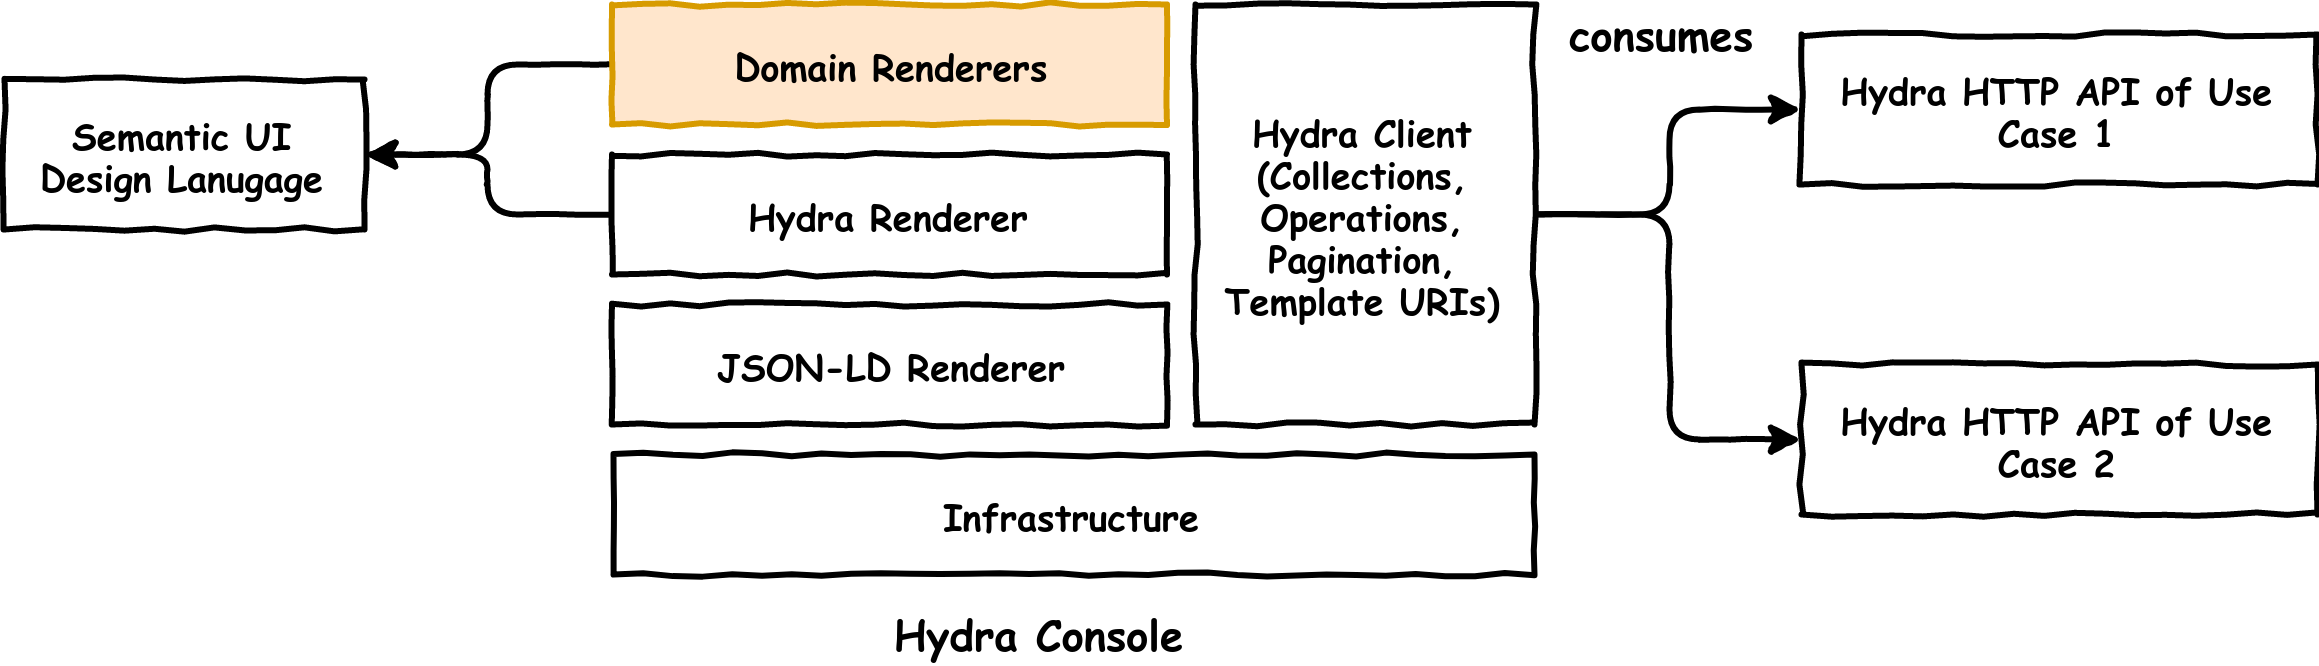
\includegraphics[width=450pt]
    {images/ui-framework-architecture.png}}
  \caption{The architecture of the proof of concept for the UI framework.}
\end{figure}

\subsection{Use Case 1: Apartment}\label{sec:usecase1}
For the user to be able to query data, the UI has to render it.

The first use case describes a scenario in home automation. Several thermometers in rooms in an apartment send the current temperature to a server. The goal is to develop a UI that displays apartments, rooms, thermometers and temperatures in a sensible manner.

\subsubsection{Requirements}

\begin{figure}[!htb]
  \center{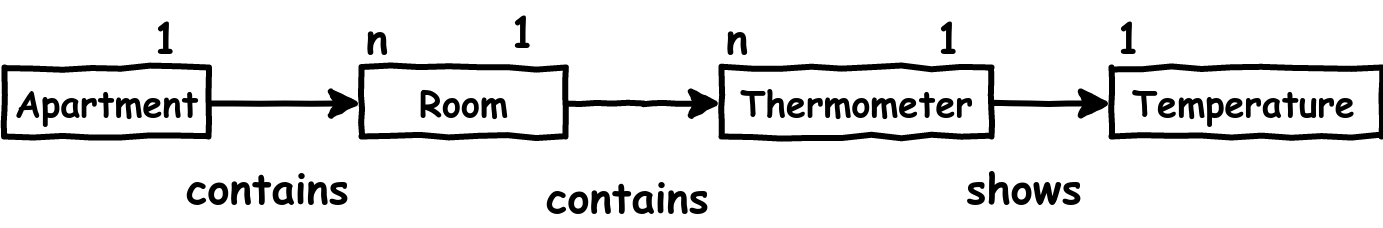
\includegraphics[width=400pt]
    {images/iot.png}}
  \caption{Data model of the apartment use case.}
\end{figure}

\begin{table}[!htb]
  \begin{center}
    \begin{tabular}{ |c|l| }
      \hline
      \textbf{ID} & \textbf{Story title} \\
      \hline
      S1 & As landlord I want to overview my apartments \\
      \hline
      S2 & As landlord I want to overview all rooms of an apartment \\
      \hline
      S3 & As landlord I want to overview thermometers of room \\
      \hline
      S4 & As landlord I want to overview the measurement data of a thermometer \\
      \hline
      S5 & As landlord I want to intuitively see the temperatures on a floor plan \\
      \hline
      S6 & As UI developer I want to present all available data without spending any development time \\
      \hline
      S7 & As UI developer I want to be able to customize the UI in order to improve it incrementally \\
      \hline
    \end{tabular}
    \caption{User stories of a scenario in home automation.}
    \label{tab:usecase1}
  \end{center}
\end{table}

\subsubsection{Hydra collection rendering}
The API exposes a collection of apartments, rooms and thermometers. Every Hydra API has an entry point and a set of root collections. These collections can be used as starting point to discover the API.

Hydra has native support for collections by using the property \lstinline{http://www.w3.org/ns/hydra/core#member}.

\lstset{language=JSON}
\begin{lstlisting}[caption=Data of /rooms as Hydra collection.]
  {
    "@context": "http://localhost:3000/iot/contexts/Room",
    "@id": "http://localhost:3000/iot/rooms",
    "@type": "Collection",
    "totalItems": 6,
    "member": [
      {
        "@id": "http://localhost:3000/iot/rooms/0",
        "@type": "https://schema.org/Room",
        "amenityFeature": "Kitchen",
        "containsPlace": [],
        "containedInPlace": "http://localhost:3000/iot/apartments/0",
        "geo": {...}
      },
      {
        "@id": "http://localhost:3000/iot/rooms/1",
        "@type": "https://schema.org/Room",
        "amenityFeature": "Laundry Storage",
        "containedInPlace": "http://localhost:3000/iot/apartments/0",
        "geo": {...}
      },
      ...
    ]
  }
\end{lstlisting}

Each member of this collection is of type \lstinline{https://schema.org/Room}. The properties can be looked up by following the URL. Given every member of the collection is of the same type, we can implement a generic renderer that looks up the properties of the member type and renders the collection as a table.

\begin{figure}[!htb]
  \center{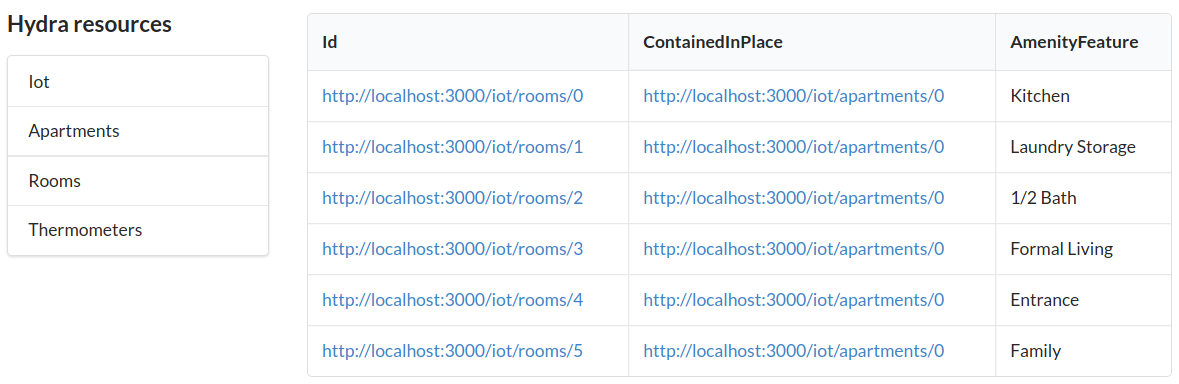
\includegraphics[width=500pt]
    {images/hydra-collections.png}}
  \caption{Generic table renderer applied on root collections.}
\end{figure}

The \lstinline{@id}s are rendered as links so that the API can be traversed by looking up resources and collections of resources.

\subsubsection{Plugin mechanism}\label{pluginmechanism}
As shown in section \ref{proofofconcept} the UI framework supports custom renderers as main mechanism to override default renderers. UI developers start out with the default set of renderers that can render arbitrary JSON-LD data and Hydra resources. \\
The fact that the API returns \gls{linkeddata} benefits this customization process. UI developers only care about rendering \textbf{certain data types}. In our use case they might be concerned with rendering the type \lstinline{Temperature}.

We demonstrate data rendering using the room \lstinline{Entrance}. The trivial JSON-LD renderer colors property keys red, properties that represent relationships blue and it renders \lstinline{@id}s as hyperlinks.

\begin{figure}[!htb]
  \center{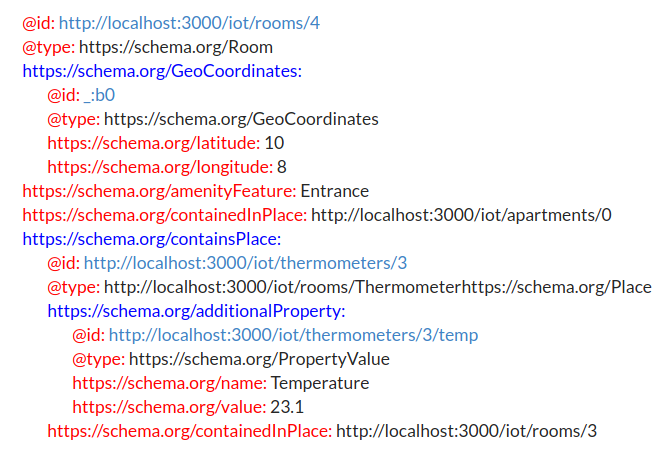
\includegraphics[width=400pt]
    {images/json-ld-renderer.png}}
  \caption{JSON-LD renderer applied on the data of \lstinline{/rooms/4}.}
\end{figure}

This room contains a list of things of type \lstinline{Thermometer} and \lstinline{https://schema.org/Place}. The thermometer has a custom \lstinline{https://schema.org/additionalProperty} that has the name \lstinline{Temperature} and a numeric value. \\
This is not straightforward to see as the JSON-LD is noisy. By applying a custom renderer to \lstinline{https://schema.org/additionalProperty} we render the temperature in one line with an icon indicating whether the temperature is hot or cold. The icon change is hard coded into the renderer.

We consider the workflow of UI developers. The UI framework expects a React component that takes the data of the \lstinline{https://schema.org/additionalProperty} and returns markup. The renderer that can be registered in the UI framework comprises of a unique id, a name, a React component and a type. The type is used by the rendering infrastructure to determine which renderers to apply on what part of the server response.

\lstset{language=JSON}
\begin{lstlisting}[caption=Renderer configuration that the developer provides.]
  {
    id: "thermometer",
    name: "Thermometer",
    comp: (data) => <Thermometer/>,
    type: "http://localhost:3000/iot/apartments/Thermometer"
  }
\end{lstlisting}

\begin{figure}[!htb]
  \center{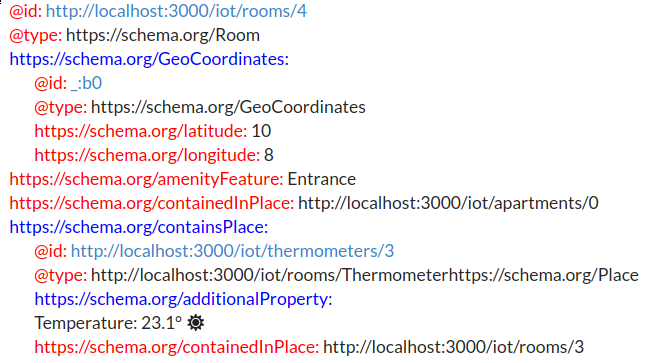
\includegraphics[width=380pt]
    {images/temperature-renderer.png}}
  \caption{The temperature renderer is applied on \lstinline{additionalProperty} on top of the JSON-LD renderer.}
  \label{fig:temperature}
\end{figure}

It is noteworthy that renderers compose by stacking them on each other. As shown in figure \ref{fig:temperature} the temperature renderer works on top the JSON-LD renderer.

By implementing similar renderers for rooms and thermometers we achieve a UI as show in figure \ref{fig:rooms}.

\begin{figure}[!htb]
  \center{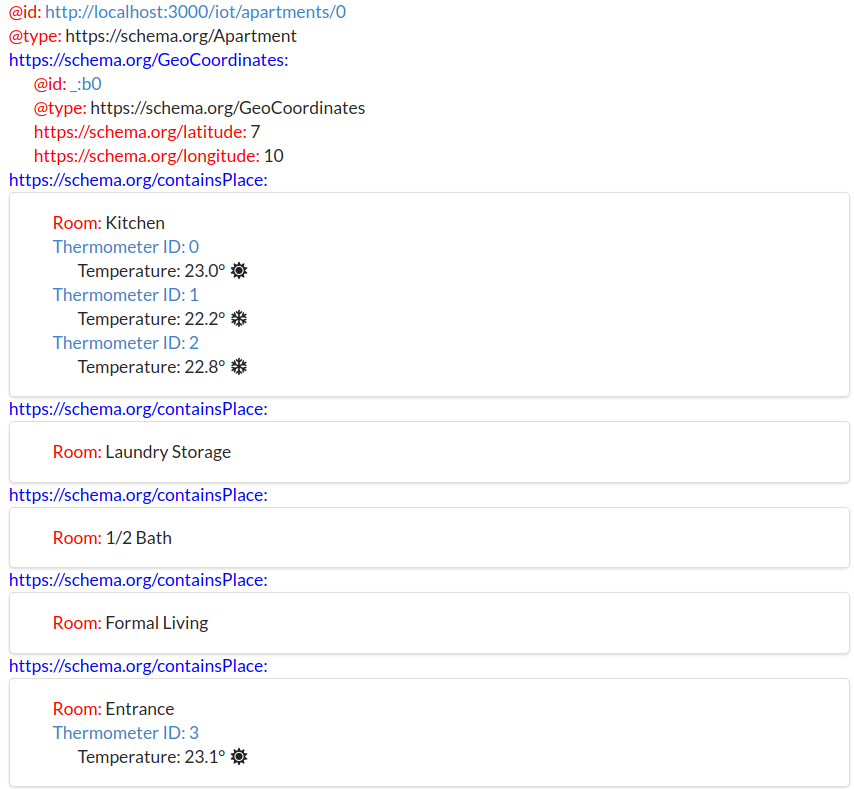
\includegraphics[width=500pt]
    {images/room-renderer.png}}
  \caption{Apartment data with active renderers: JSON-LD, Thermometer, Temperature, Room.}
  \label{fig:rooms}
\end{figure}

\subsubsection{Domain rendering}
Both default renderers are registered using the plugin mechanism. Activating both leads to a UI that is correct \footnote{Here we use the term correct in the sense of correct data rendering - the UI doesn't show wrong or non-existing data and it shows all of the response data.} and the user is able to navigate through the API using hyperlinks. This rendering setup is decoupled from the API implementation but the API has to conform to the the Hydra specification.

In order to leverage domain information for visualizing data, UI developers have to provide custom components that contain domain knowledge. We demonstrate domain rendering by looking at one apartment.

The thermometer renderer removes some noise by compacting the thermometer data. The room renderer removes some properties that are not important in this context and it draws a box around the room so they are easier to distinguish. This list view provides all information to the landlord that he cares about. \\
Places and containment relationships of places can be visualized in a more intuitive way.

\paragraph{Floor plan}
The apartment has a property called \lstinline{https://schema.org/hasMap}.

\lstset{language=JSON}
\begin{lstlisting}[caption=The \lstinline{hasMap} property of apartment /apartments/0.]
...
  "hasMap": {
  "@type": "https://schema.org/URL",
  "@id": "http://localhost:3000/iot/floorplan.jpg"
}
...
\end{lstlisting}

This property has a link to an image representing the floor plan of the apartment.

\paragraph{Geo coordinates}
All things of type \lstinline{https://schema.org/Apartment} and \lstinline{https://schema.org/Room} can have a \lstinline{geo} property.

\lstset{language=JSON}
\begin{lstlisting}[caption=The \lstinline{https://schema.org/geo} property of apartment /apartments/0.]
...
  "geo": {
    "@type": "https://schema.org/GeoCoordinates",
    "longitude": 10,
    "latitude": 7
  }
...
\end{lstlisting}

This property contains the longitude and latitude coordinates of the center of the place.

Both properties \lstinline{https://schema.org/hasMap} and \lstinline{https://schema.org/geo} are defined on the type \lstinline{https://schema.org/Place}. \lstinline{https://schema.org/Apartment} is a subtype of \lstinline{https://schema.org/Place} in the schema.org hierarchy, so our apartment renderer assumes the existence of those properties.

By leveraging coordinates of places and the floor plan of the apartment we use domain knowledge to implement a renderer that provides additional value to the landlord. By rendering the rooms on the floor plan the landlord can grasp the locations of thermometers in a more natural way.

\begin{figure}[!htb]
  \center{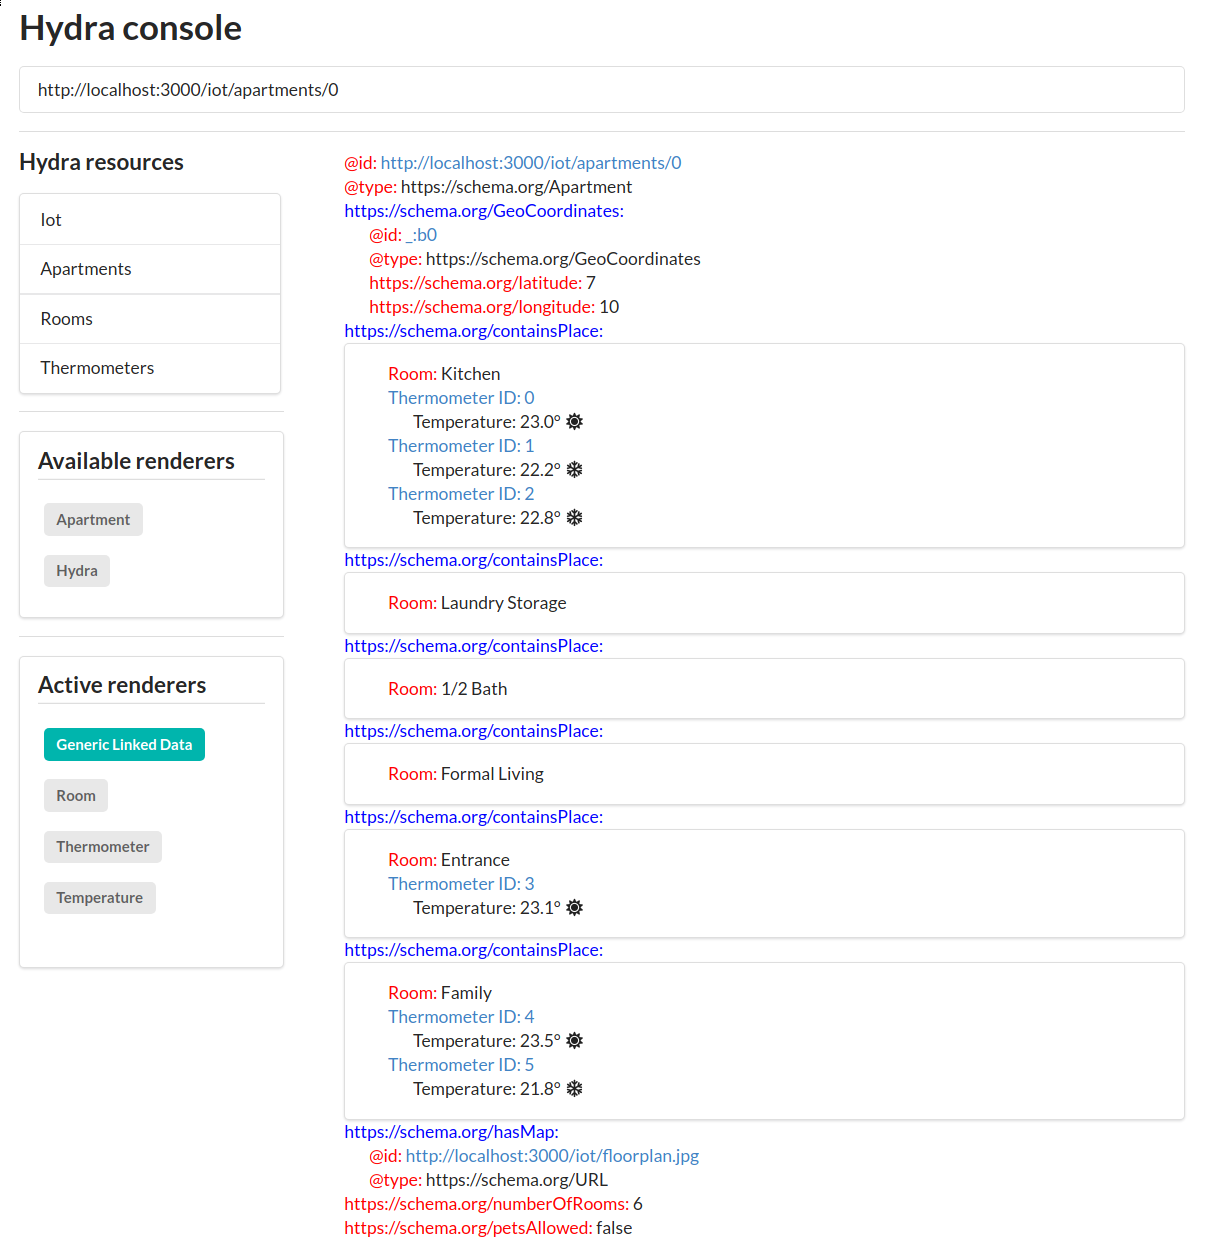
\includegraphics[width=500pt]
    {images/apartment-renderer.png}}
  \caption{Apartment data with active renderers: JSON-LD, Thermometer, Temperature, Room, Apartment, BoldFont.}
  \label{fig:apartmentrenderer}
\end{figure}

It is noteworthy that a set of renderers can be active at the same time. Whenever the rendering infrastructure encounters a data type that has a registered renderer it will apply it. In this example Hydra collections are still rendered as tables if the landlord opens the collection of rooms or thermometers.

\subsubsection{Verification of user stories}
In this section we verify that the user stories listed in table \ref{tab:usecase1} are fulfilled by either accepting or rejecting them.

\begin{table}[!htb]
  \begin{center}
    \begin{tabular}{ |l|l| }
      \hline
      \textbf{ID} & \textbf{Outcome} \\
      \hline
      S1 & Accepted: The landlord can overview the apartments \\
      \hline
      S2 & Accepted: The landlord can list all rooms of an apartment \\
      \hline
      S3 & Accepted: The landlord can list all thermometers of a rooms \\
      \hline
      S4 & Accepted: The landlord can see the temperature reported by a thermometer \\
      \hline
      S5 & Accepted: The landlord can overview the location of the temperatures on the floor plan \\
      \hline
      S6 & Accepted: The UI developer uses the default renderers to render a correct UI \\
      \hline
      S7 & Accepted: The UI developer can register custom renderers to improve the UI incrementally \\
      \hline
    \end{tabular}
    \caption{All user stories are accepted and the first use case is implemented.}
  \end{center}
\end{table}

\subsection{Use Case 2: Kanban Board}
The second use case describes a typical scenario in project management. We use this use case to explore the viability of Hydra for UIs with user interaction. A project has multiple issues which represent chunks of work. Issues can be in one of the following statuses:

\subsubsection{Requirements}

\begin{enumerate}
  \item Backlog: Status of an issue that needs additional input before it can be worked on.
  \item Ready: Status of an issue that has well defined requirements - enough information is available to start implementation.
  \item In process: Status of an issue that is being worked on.
  \item Done: Status of an issue that has been implemented.
\end{enumerate}

\begin{figure}[!htb]
  \center{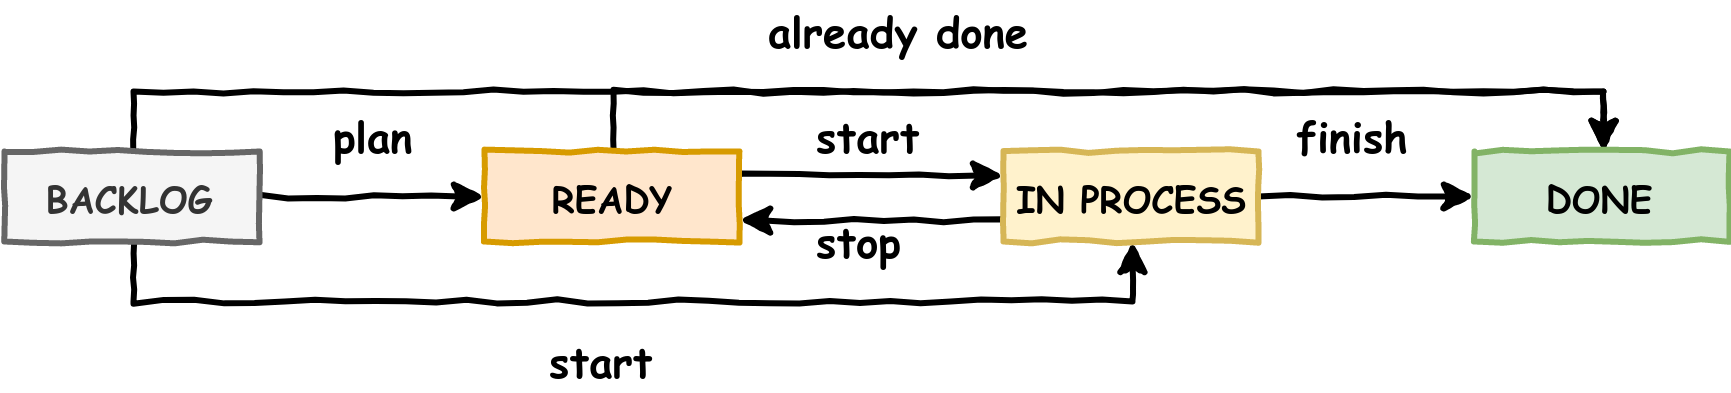
\includegraphics[width=400pt]
    {images/state-diagram.png}}
  \caption{Status transitions of an issue.}
  \label{fig:statetransition}
\end{figure}

Figure \ref{fig:statetransition} shows all possible statuses and status transitions of an issue. It is noteworthy that once an issue is ready, it can not be put back to the backlog and similarly a finished issue can not be undone.

\begin{figure}[!htb]
  \center{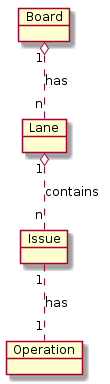
\includegraphics[width=150pt]
    {images/kanban.png}}
  \caption{Simple data model of a scenario in project management.}
\end{figure}

\begin{table}[!htb]
  \begin{center}
    \begin{tabular}{ |l|l| }
      \hline
      \textbf{ID} & \textbf{Story title} \\
      \hline
      S1 & As project manager I want to overview all projects \\
      \hline
      S2 & As project manager I want to overview all issues of a project \\
      \hline
      S3 & As project manager I want to see the status of an issue \\
      \hline
      S4 & As project manager I want to change the status of an issue \\
      \hline
      S5 & As project manager I want to remove issues \\
      \hline
      S6 & As a project manager I want to change the issue status by drag and drop \\
      \hline
      S7 & As UI developer I want to present all available data without spending time \\
      \hline
      S8 & As UI developer I want to be able to customize the UI in order to improve it incrementally \\
      \hline
      S9 & As UI developer I want to have an interactive UI without spending time \\
      \hline
    \end{tabular}
    \caption{User stories of a scenario in project management.}
    \label{tab:usecase2}
  \end{center}
\end{table}

\subsubsection{User interaction}
Hydra supports user interaction through operations. The server tells the client how to build an operation which the client then can invoke. Hydra supports three types of operations:

\paragraph{Inline operations}
The actual data is augmented with a list of supported operations. The resource has a property \lstinline{supportedOperations} where the resource is the operation object \footnote{The subject invokes the operation on an object}.

\paragraph{Attached to supported properties}
Hydra supports documentation of properties. The documentation can include information about which values are valid for a property. It is possible to attach operations to those properties.

\paragraph{Attached to supported classes}
Similar to the concept of supported properties, it is possible to document classes. Classes are used to group things together that are used the same way in certain contexts. Classes can be assigned to things by using the \lstinline{@type} property.

We attach supported operations to supported classes of issues that represent issue statuses.

\subsubsection{State transition as Hydra operations}
This section discusses the HTTP API implementation of the issue status change actions. The goal is to implement the state transition shown in figure \ref{fig:statetransition}.

\paragraph{Hydra classes}\label{par:classes}
Each status that has outgoing state transitions maps to a Hydra class. We have the classes \lstinline{BacklogIssue}, \lstinline{ReadyIssue}, \lstinline{InProcessIssue}. Note that there is no class for an issue that is done because according to the status transitions there is no way to change the status of such an issue.

Each \textbf{out} going status transition is represented by a Hydra class as well. Our API documentation contains \lstinline{IssueToReadyUpdate}, \lstinline{IssueToInProcessUpdate}, \lstinline{IssueToDoneUpdate} as additional classes. There is no \lstinline{IssueToBacklogUpdate}, because according to the state transitions, it is not possible to undo planned issues.

\paragraph{Supported operations}
Each issue class supports a list of operations.

\begin{table}[!htb]
  \begin{center}
    \begin{tabular}{ |c|l| }
      \hline
      \textbf{Status class} & \textbf{Operation classes} \\
      \hline
      BacklogIssue & IssueToReadyUpdate, IssueToInProcessUpdate, IssueToDoneUpdate \\
      \hline
      ReadyIssue & IssueToInProcessUpdate, IssueToDoneUpdate \\
      \hline
      InProcessIssue & IssueToReadyUpdate, IssueToDoneUpdate \\
      \hline
    \end{tabular}
    \caption{Status transition matrix.}
    \label{tab:statetransitionmatrix}
  \end{center}
\end{table}

Translation of the state transition diagram \ref{fig:statetransition} and mapping of the Hydra classes defined in \ref{par:classes} to the states and state transitions leads to the state transition matrix shown in \ref{tab:statetransitionmatrix}.

\lstset{language=JSON}
\begin{lstlisting}[caption=Exempt of the Hydra documentation showing the list of supported operations for the issue status class ReadyIssue.]
  ...
  {
    "@id": "http://localhost:3000/kanban/issues/ReadyIssue",
    "@type": "Class",
    "title": "Issue that is ready",
    "description": "An issue which is ready and can be started.",
    "supportedOperation": [
      {
        "@type": "http://schema.org/UpdateAction",
        "method": "POST",
        "label": "Start",
        "expects": "http://localhost:3000/kanban/issues/IssueToInProcessUpdate",
        "returns": null
      },
      ...
    ]
  },...
\end{lstlisting}

\subsubsection{Generically rendering operations}
Similar to the first use case in \ref{sec:usecase1} the list of issues is rendered using the \textit{Hydra renderer}. The properties of an issue \lstinline{description} and \lstinline{title} are columns in a table. The last column is used for Hydra operations in case any of the issues (table rows) has at least one supported operation.

Operations have an HTTP \lstinline{method} property so the client knows how to invoke that operation. We use this information to render buttons for issue removal and issue status change differently.

\begin{figure}[!htb]
  \center{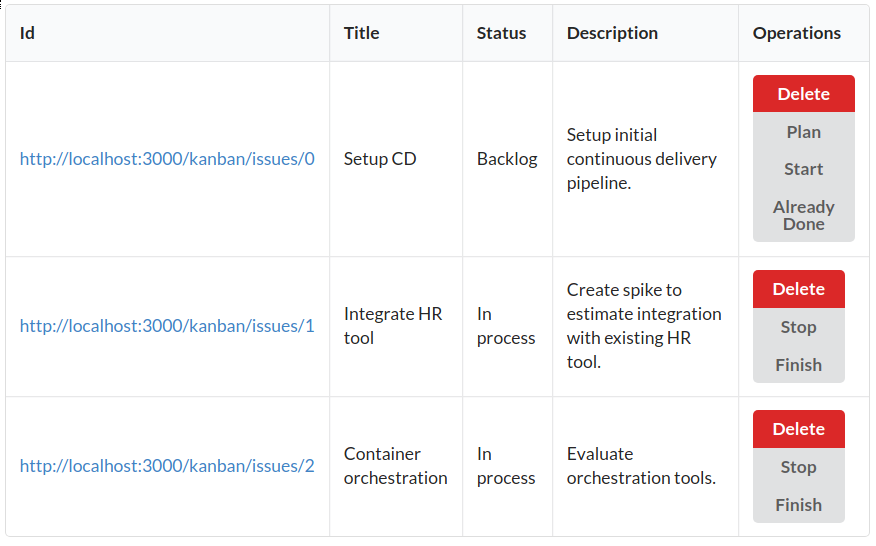
\includegraphics[width=470pt]
    {images/issues-hydra-renderer.png}}
  \caption{Collection of issues rendered by the Hydra renderer.}
  \label{fig:issueshydra}
\end{figure}

A click on a start status change button, shown in \ref{fig:issueshydra}, causes the Hydra client to invoke the operation. The client fetches \lstinline{http://localhost:3000/kanban/issues/IssueToInProcessUpdate} and sends a POST request to the URL of the issue in that row.

\subsubsection{Domain rendering}
Using the plugin mechanism mentioned in section \ref{pluginmechanism} we implement a domain specific renderer that interprets this list of issues as a Kanban \footnote{Project scheduling methodology, issue cards that move through production/development stages.} board. Figure \ref{fig:kanban} shows issues grouped by their statuses on a Kanban board.

\begin{figure}[!htb]
  \center{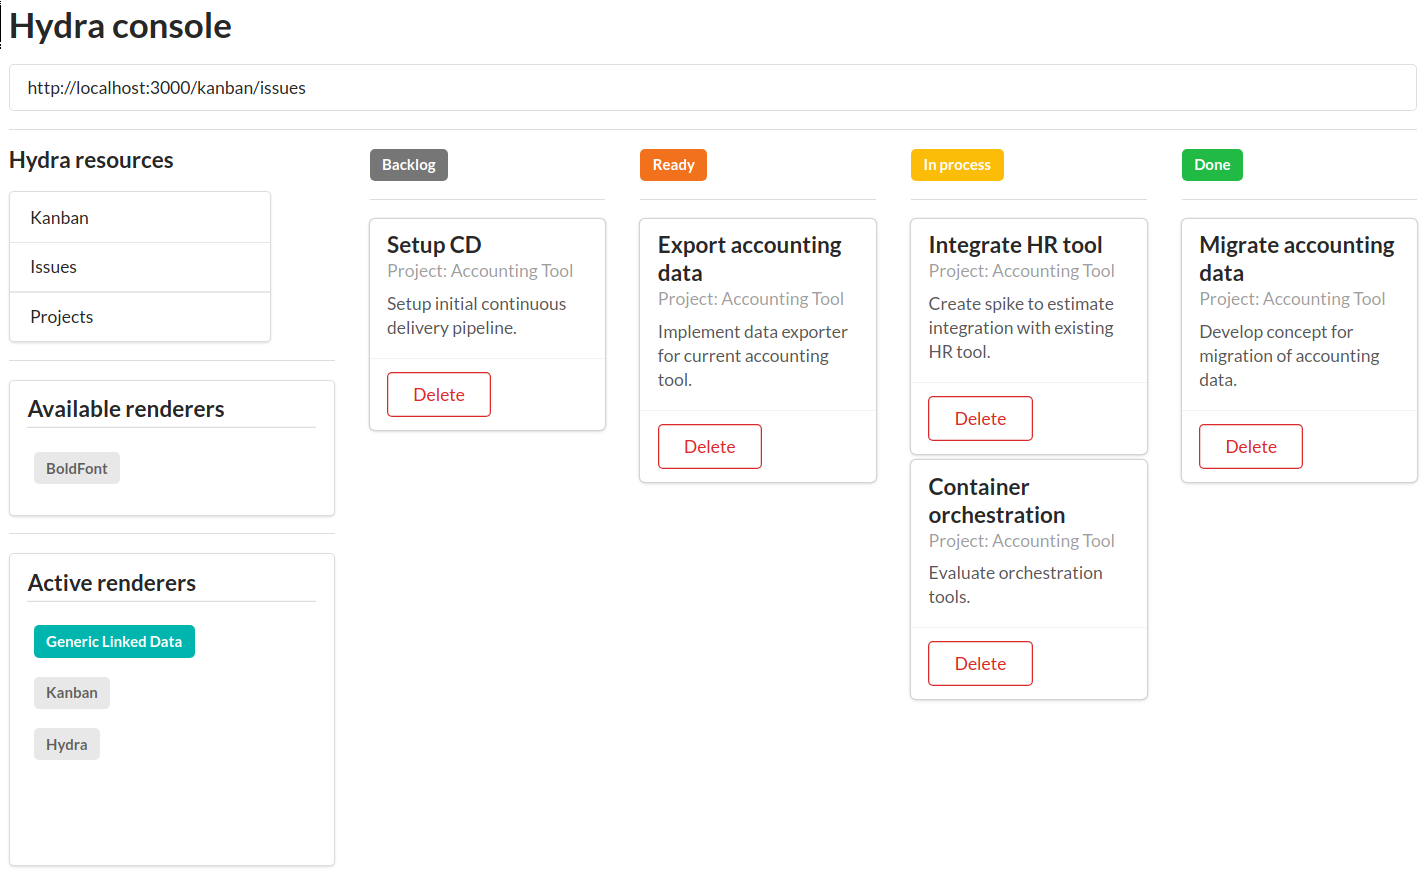
\includegraphics[width=470pt]
    {images/kanban-renderer.png}}
  \caption{Collection of issues rendered by the domain specific Kanban renderer.}
  \label{fig:kanban}
\end{figure}

\paragraph{Intuitive status change}
The Kanban renderer consumes supported operations per issue and let's the project manager invoke them in an intuitive way. The look and feel of an issue implies that it can be dropped on the target status. The visual grouping by status helps the project manager to quickly see what the development team is working on.

\paragraph{Optimistic rendering}
Optimistic rendering tries to hide the latency of the request-response life cycle. Instead of awaiting the positive response of the server confirming operation success the client behaves as if the positive response was immediate. This approach only works for operations that are expected to succeed most of the time.

For idempotent \footnote{Idempotence is a property of an operation that can be applied multiple times without changing the result beyond the initial application, in HTTP PUT and DELETE are idempotent where POST is not.} HTTP methods like \lstinline{PUT} or \lstinline{DELETE} it is possible to generically implement optimistic rendering \textbf{that works most of the time}. When the project manager for instance removes an issue, the object of the operation is known. The client immediately removes the issue from the UI without waiting for confirmation. When implementing optimistic rendering, one has to make sure to handle operation failures in a sensible way. \\
We consider the erroneous case where the project manager removes an issue and it reappears after a few hundred milliseconds. In the worst case, he doesn't pay attention after clicking the delete button and goes on thinking that the issue has been removed. This is the reason one has to carefully design optimistic rendering - especially the negative scenario. Often, it is not possible or feasible to implement optimistic rendering in a generic way.

The Kanban renderer can leverage domain knowledge to implement optimistic rendering. It simply appends the issue item to the list of issues in a column. It has knowledge of vertically aligned issue items where the Hydra renderer just knows about collections of issues. Impossible in going state transitions are communicated by not allowing issues to be dropped on the \lstinline{Backlog} column. Impossible out going state transitions are communicated by not allowing the project manager to pick up an issue that is \lstinline{Done}.

\subsubsection{Verification of user stories}
In this section we verify that the user stories listed in table \ref{tab:usecase2} are fulfilled by either accepting or rejecting them.

\begin{table}[!htb]
  \begin{center}
    \begin{tabular}{ |c|l| }
      \hline
      \textbf{ID} & \textbf{Outcome} \\
      \hline
      S1 & Accepted: The project manager can overview all projects \\
      \hline
      S2 & Accepted: The project manager can overview all issues of a project \\
      \hline
      S3 & Accepted: The project manager can see the status of an issue \\
      \hline
      S4 & Accepted: The project manager can see the status of an issue \\
      \hline
      S5 & Accepted: The project manager can remove issues \\
      \hline
      S6 & Accepted: The project manager can drag and drop issues \\
      \hline
      S7 & Accepted: The Hydra renderer shows all data \\
      \hline
      S8 & Accepted: The UI developer can override the generic renderers \\
      \hline
      S9 & Accepted: The Hydra renderer exposes all operations by default \\
      \hline
    \end{tabular}
    \caption{All user stories are accepted and the second use case is implemented.}
  \end{center}
\end{table}

\subsection{Result}
By implementing a simple dashboard for home automation and a simple Kanban board for project management, we have developed the proof of concept for the UI framework. It provides generic rendering capabilities out of the box using the JSON-LD and Hydra renderers. Those can be overridden by custom React components provided by the UI developer. Custom renderers define which \lstinline{@type}s they can render - the infrastructure takes care of rendering.

\begin{figure}[!htb]
  \center{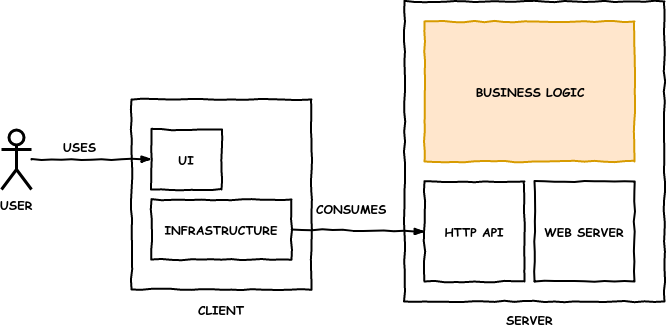
\includegraphics[width=380pt]
    {images/ui-dev.png}}
  \caption{Solely the server contains business logic.}
  \label{fig:businesslogic}
\end{figure}

Neither the client nor the custom renderers contain business rules whatsoever. The custom renderers might contain knowledge on how to present business types, but the client is merely a \gls{console} to the Hydra API as shown in figure \ref{fig:businesslogic}.

\begin{figure}[!htb]
  \center{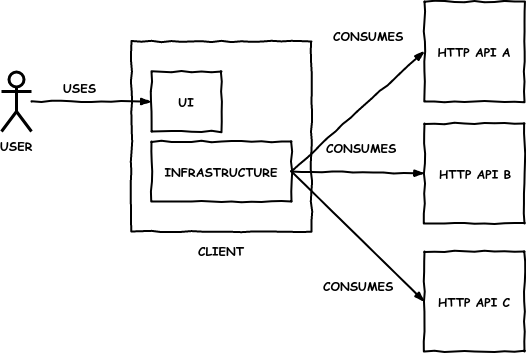
\includegraphics[width=380pt]
    {images/client-instances.png}}
  \caption{The client is decoupled from any API and is able to consume different APIs.}
  \label{fig:losecoupling}
\end{figure}

This lose coupling between client and API implementation allows the same client to be used for various API implementations as shown in figure \ref{fig:losecoupling}.

\begin{figure}[!htb]
  \center{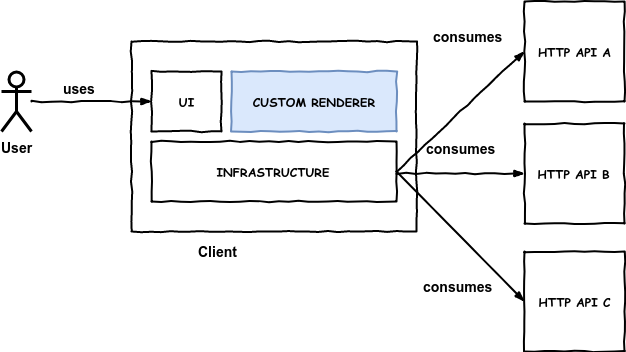
\includegraphics[width=380pt]
    {images/ui-dev-custom-renderer.png}}
  \caption{Custom renderers provide the ability to render data types. By avoiding hard coding business logic into the client the coupling to the server is still loose.}
  \label{fig:linkeddata}
\end{figure}

By using \gls{linkeddata}, custom renderers don't affect reusability of the client. A context is provided by \gls{linkeddata} so it can be understood by machines. That context is not hard coded into the client like it is often done in contemporary UI development. \\
To elaborate, we look at figure \ref{fig:linkeddata} and assume that a custom renderer for the type \lstinline{https://schema.org/Apartment} is implemented. If the responses of API A, API B and API C contain data with \lstinline{@type} \lstinline{https://schema.org/Apartment} the client can consume that data. \\
Sometimes it is required to display data differently depending on the UI context. The apartment might be rendered differently in a back office application used by administrators than an end-user facing website that lists apartments nearby. The underlying data is the same, the rendered apartment is different. This has to be resolved on the data modeling level by using Hydra classes. Classes can be used to apply additional \lstinline{@type}s depending on the context of the UI.

\section{Results}\label{sec:results}
In the following paragraph we evaluate the proof of concept for the UI framework. We examine whether the design goals have been met and we analyze the change in complexity.

\subsection{Methodology}
In order to evaluate the UI framework and its concepts we are using two scoring systems. To asses whether goals have been met, scores between 0 and 3 are assigned as described in table \ref{tab:designgoalsscore}. To gauge how complexity has been affected we use scores between -3 and 3 as shown in table \ref{tab:complexityscore}. \\
Finally, we list remarkable findings that came up during development of the proof of concept, during the usage of it or during the usage of the resulting UI.

\begin{table}[!htb]
  \begin{center}
    \begin{tabular}{|l|l|}
      \hline
      \textbf{Score} & \textbf{Effect on goal} \\
      \hline
      0 & The goal is not met \\
      \hline
      1 & Slight improvement towards goal \\
      \hline
      2 & The design goal is mostly met \\
      \hline
      3 & The design goal is completely fulfilled \\
      \hline
    \end{tabular}
    \caption{Scale to asses whether a design goal was met.}
    \label{tab:designgoalsscore}
  \end{center}
\end{table}

\begin{table}[!htb]
  \begin{center}
    \begin{tabular}{|l|l|}
      \hline
      \textbf{Score} & \textbf{Effect on complexity} \\
      \hline
      -3 & Massive increase in complexity \\
      \hline
      -2 & Increase in complexity \\
      \hline
      -1 & Slight increase in complexity \\
      \hline
      0 & No change in complexity \\
      \hline
      1 & Slight decrease in complexity \\
      \hline
      2 & Decrease in complexity \\
      \hline
      3 & Massive decrease in complexity \\
      \hline
    \end{tabular}
    \caption{Scale of the effect on complexity by using the UI framework.}
    \label{tab:complexityscore}
  \end{center}
\end{table}

\subsection{Design goals}
By looking at the implementations of both use cases, we evaluate whether the design goals defined in \ref{sec:designgoals} have been met.

\subsubsection{Play nicely with others}
Playing nicely with other technologies, existing consumers and existing tooling is the major design goal as described in section \ref{sec:playnice}. Choices on the technologies being used in the UI framework have the biggest impact on it.

\paragraph{JSON-LD}
JSON-LD is valid JSON - any tool that accepts JSON also accepts JSON-LD.

\paragraph{Hydra operations}
Hydra operations include an  HTTP verb which the client reads to invoke the operation. Given the developer respects the conventions regarding safe and idempotent HTTP verbs, their invocations are equal to regular HTTP requests. HTTP proxies and caches treat Hydra requests the same as other HTTP requests.

\paragraph{React}
As discussed in section \ref{sec:react}, React is one of the widely used tools for UI development. The proof of concept for the UI framework accepts only custom renderers using React components. \\
HTML templates \citep{htmltemplates}, which are part of the Web component specification, might become a better choice for the DOM rendering component once the tooling has developed.

\paragraph{Summary}
Due to choice of technology this design goal has been fulfilled and we assess it with a \textbf{score of 3}.

\subsubsection{Straightforward upgrade path}
We assume a scenario with a running RESTful HTTP API returning JSON and a client consuming it. The client renders the UI with a custom rendering solution that creates the DOM based on input data. API documentation is generated using a custom tool and the documentation is served using another server. The development team evaluates the upgrade path to a Hydra conform API using the UI framework. We discuss the upgrade steps to evaluate if the upgrade path is straightforward and to asses the amount of friction.

\paragraph{Entity serialization}
Serialization of entities to Hydra resources remains the same. Adding a header that transmits the context, similar to the \lstinline{@context} property, suffices. The response payload remains the same and existing consumers don't break.

\paragraph{Hydra documentation}
Documentation is served using the meta data mechanism of Hydra. The response header points to the documentation of the requested resource. The existing API documentation is marked as deprecated. Developers use the Hydra documentation instead of the old one, the previous solution can be removed after a grace period.

\paragraph{Hydra operations}
As the current API follows RESTful principles, the concepts of resources and HTTP methods exist. Resources and HTTP methods are directly mapped to Hydra resources and inline operations using the same HTTP method. This change requires careful design as it might break existing consumers. Migrating existing HTTP methods to Hydra in a non-breaking way might lead to a non-idiomatic use of Hydra operations. This approach could serve as a stepping stone towards using the features of Hydra to its full extent.

\paragraph{Summary}
Due to choice of HATEOAS specification and \gls{linkeddata} format, it is almost straightforward to upgrade existing RESTful APIs returning JSON. The \textbf{score is 2.5}.

\subsubsection{Customizability}
In order to assess the customizability of the UI framework, we compare the set of UIs that can be implemented using the UI framework with the set of UIs that can be implemented using tools like React.

\paragraph{Plugin mechanism}
The plugin mechanism allows UI developers to map components to data types. It is possible to register a renderer using the wildcard \lstinline{*} type. This activates the renderer on every type. UI developers can take control over rendering by using wildcards to render a React component with all the response data as input. The set of UIs that can be implemented using the UI framework is equal to the set of UIs that can be implemented using React.

\paragraph{Summary}
This design goal is fulfilled which leads to a \textbf{score of 3}.

\subsubsection{Developer ergonomics}
We analyze the usage of the UI framework by a developer.

\paragraph{Component API}
Every React component that is invoked by the rendering infrastructure gets a Hydra resource and a \lstinline{renderer} function as input.

\lstset{language=JSON}
\begin{lstlisting}[caption={React component API for the apartment renderer as shown in figure \ref{fig:apartmentrenderer}.}, label={lst:componentapi}]
  const Apartment = ({resource, renderer}) => {
    const { "https://schema.org/containsPlace": rooms } = resource;
    return (
      <div style={{ position: "relative" }}>
        ...
        {rooms.map((r: any) => {
          return (
            <PositionedRoom
              renderer={renderer}
              data={r}
              key={r["@id"]}
              xPos={xPos}
              yPos={yPos}
            />
            );
        })}
      </div>
    )
  }
\end{lstlisting}

Listing \ref{lst:componentapi} shows the apartment renderer of the apartment use case. The \lstinline{resource} contains the data of the Hydra resource of \lstinline{@type} \lstinline{https://schema.org/Apartment}. It accesses the property \lstinline{https://schema.org/containsPlace} to fetch the rooms of the apartment. The \lstinline{renderer} function can be invoked with a Hydra resource. This returns the control of the rendering process to the rendering infrastructure.

This allows UI developers to think in terms of data types and self-contained components. Developing isolated components without thinking about mapping data to children components reduces \gls{cognitive load}.

\paragraph{Learning curve}
The learning curve of the UI framework is equals roughly the sum of the learning curves of JSON-LD, React and Hydra. The knowledge required to create and register custom renderers is trivial and can be neglected in this discussion. \\
Superficial knowledge about JSON-LD is sufficient to use the UI framework. If the developer is only concerned with rendering non-interactive UIs, knowledge about the two special JSON-LD properties like \lstinline{@type} and \lstinline{@id} is enough. \\
Although Alcaeus \footnote{\url{https://github.com/wikibus/Alcaeus}} hides implementation details of Hydra, UI developers should know about operations, classes, documentation and collections in order to create interactive UIs. Deep understanding of Hydra and the Hydra client Alcaeus are required for debugging. \\
The learning curve of using React with the UI framework is flat compared to using React standalone. The developer doesn't have to care about topics like state management and client side routing. React has a mature ecosystem of tools covering these topics - their use comes with cognitive overhead. Using the UI framework, developers can focus on learning React without being concerned with those topics.

\paragraph{Summary}
The learning curve to implement non-interactive UIs is minimal. The component API and renderer registering are simple - the developer can focus on non-infrastructure topics. Implementing and debugging interactive UIs requires a high level of understanding of Hydra. We assess the score of developer ergonomics \textbf{to be 2}.

\subsubsection{Summary}

\begin{table}[!htb]
  \begin{center}
    \begin{tabular}{|l|l|l|}
      \hline
      \textbf{ID} & \textbf{Title} & \textbf{Degree to which goal is met} \\
      \hline
      D1 & Play nicely with others & 3 \\
      \hline
      D2 & Straightforward upgrade path & 2.5 \\
      \hline
      D3 & Customizability & 3 \\
      \hline
      D4 & Developer ergonomics & 2 \\
      \hline
    \end{tabular}
    \caption{Overview of the design goals and their score indicating the degree to which they are met.}
    \label{tab:designgoalscomplexity}
  \end{center}
\end{table}

\subsection{Reduction of complexity in software development}
This section analyzes whether and how development with the UI framework affects various types of software complexity. This requires a comparison of a traditional ``non'' \gls{linkeddata}-driven approach to the development workflow using the UI framework.

\paragraph{Baseline scenario} We describe a baseline scenario where a development team is working on a RESTful HTTP API that returns JSON and on a \gls{frontend} using React. They use Swagger \footnote{Swagger is a tool for documentation and development of HTTP APIs. \url{https://swagger.io/}} to generate and serve API documentation.

We assess various types of software complexities in order to gauge the change in complexity from the baseline scenario to scenario using the UI framework and Hydra. We assume that a change in software complexity is a similar change in software development cost.

\subsubsection{Essential Complexity}
Brooks gives \textit{Complexity}, \textit{Conformity}, \textit{Changeability} and \textit{Invisibility} as the four properties of software causing Essential Complexity \citep{nosilverbullet}.

\paragraph{Complexity caused by Invisibility}
\textit{``Software is invisible and unvisualizable. Geometric abstractions are powerful tools. The floor plan of a building helps both architect and client evaluate spaces, traffic flows, views. Contradictions and omissions become obvious. Scale drawings of mechanical parts and stick-figure models of molecules, although abstractions, serve the same purpose. A geometric reality is captured in a geometric abstraction. \\ The reality of software is not inherently embedded in space. Hence, it has no ready geometric representation in the way that land has maps, silicon chips have diagrams, computers have connectivity schematics. As soon as we attempt to diagram software structure, we find it to constitute not one, but several, general directed graphs superimposed one upon another. The several graphs may represent the flow of control, the flow of data, patterns of dependency, time sequence, name-space relationships. These graphs are usually not even planar, much less hierarchical. Indeed, one of the ways of establishing conceptual control over such structure is to enforce link cutting until one or more of the graphs becomes hierarchical.''} \citep[p.~4]{nosilverbullet}

The development team starting out with the Hydra API and the UI framework is able to render a fully functional UI without spending any development effort. JSON-LD is rendered as a tree and relationships between resources are apparent. The Hydra renderer displays collections of data as tables. In the baseline scenario developers have to spend a considerable amount of effort on infrastructure before they can render tables. The UI framework \textbf{increases visibility slightly} by providing these visualizations out of the box.

We asses the improvement in complexity caused by Invisibility with a \textbf{score of 1}.

\paragraph{Complexity caused by Conformity}
\textit{''Software people are not alone in facing complexity. Physics deals with terribly complex objects even at the "fundamental" particle level. The physicist labors on, however, in a firm faith that there are unifying principles to be found, whether in quarks or in unifiedfield theories. Einstein argued that there must be simplified explanations of nature, because God is not capricious or arbitrary. \\ No such faith comforts the software engineer. Much of the complexity that he must master is arbitrary complexity, forced without rhyme or reason by the many human institutions and systems to which his interfaces must conform. These differ from interface to interface, and from time to time, not because of necessity but only because they were designed by different people, rather than by God. \\ In many cases, the software must conform because it is the most recent arrival on the scene. In others, it must conform because it is perceived as the most conformable. But in all cases, much complexity comes from conformation to other interfaces; this complexity cannot be simplified out by any redesign of the software alone.''} \citep[p.~3]{nosilverbullet}

The UI framework doesn't affect the complexity that emerges from this property.

The \textbf{score is 0}.

\paragraph{Complexity caused by Changeability}
\textit{``The software entity is constantly subject to pressures for change. Of course, so are buildings, cars, computers. But manufactured things are infrequently changed after manufacture; they are superseded by later models, or essential changes are incorporated into later-serial-number copies of the same basic design. Call-backs of automobiles are really quite infrequent; field changes of computers somewhat less so. Both are much less frequent than modifications to fielded software. \\ In part, this is so because the software of a system embodies its function, and the function is the part that most feels the pressures of change. In part it is because software can be changed more easily - it is pure thought-stuff, infinitely malleable. Buildings do in fact get changed, but the high costs of change, understood by all, serve to dampen the whims of the changers.''} \citep[p.~4]{nosilverbullet}

The custom domain renderers are valid in a broader context because they consume \gls{linkeddata}. The UI remains functional as long as the HTTP API conforms to the Hydra specification. By design, it is possible to change the HTTP API within those boundaries while a user is interacting with the UI - without breaking the UI.

The cost of change in the client and the UI is \textbf{drastically} reduced. \textbf{The score of the improvement is 3}.

\paragraph{Complexity caused by Complexity}
\textit{``The complexity of software is an essential property, not an accidental one. Hence, descriptions of a software entity that abstract away its complexity often abstract away its essence. For three centuries, mathematics and the physical sciences made great strides by constructing simplified models of complex phenomena, deriving properties from the models, and verifying those properties by experiment. This paradigm worked because the complexities ignored in the models were not the essential properties of the phenomena. It does not work when the complexities are the essence.''} \citep[p.~3]{nosilverbullet}

The gist of this property is that complexity breeds complexity. If a software system becomes complex, it becomes harder to add new components without code duplication. Due to the existing complexity it might be hard to understand the code. \\ Decreasing the complexity by reducing the impact of the other three properties improves this point by definition.

This software property is not orthogonal to the other three. It is not possible to gauge the effect on complexity caused by complexity using the UI framework.

\paragraph{Summary}
While it is not possible to get rid of these properties of software, the UI framework reduces their impact on complexity in the development process. The data that is driving the client and the UI is visualized by default and the \textbf{complexity of changing the client is massively decreased}.

\subsubsection{Accidental Complexity}
\textit{Out of the Tar Pit} identifies \textit{Complexity of State} and \textit{Complexity of Control} as concrete types of Accidental Complexity by building on top of the work of Brooks.

\paragraph{Complexity caused by State}
\textit{``The severity of the impact of state on testing noted by Brooks is hard to over-emphasise. State affects all types of testing — from system-level testing (where the tester will be at the mercy of the same problems as the hapless user just mentioned) through to component-level or unit testing. The key problem is that a test (of any kind) on a system or component that is in one particular state tells you nothing at all about the behaviour of that system or component when it happens to be in another state. \\ The common approach to testing a stateful system (either at the component or system levels) is to start it up such that it is in some kind of “clean” or “initial” (albeit mostly hidden) state, perform the desired tests using the test inputs and then rely upon the (often in the case of bugs ill-founded) assumption that the system would perform the same way - regardless of its hidden internal state - every time the test is run with those inputs.''} \citep[p.~6]{outoftarpit}

\textit{``In addition to causing problems for understanding a system from the outside, state also hinders the developer who must attempt to reason (most commonly on an informal basis) about the expected behaviour of the system “from the inside”. \\ The mental processes which are used to do this informal reasoning often revolve around a case-by-case mental simulation of behaviour: “if this variable is in this state, then this will happen - which is correct - otherwise that will happen 0 which is also correct”. As the number of states - and hence the number of possible scenarios that must be considered - grows, the effectiveness of this mental approach buckles almost as quickly as testing (it does achieve some advantage through abstraction over sets of similar values which can be seen to be treated identically). \\ One of the issues (that affects both testing and reasoning) is the exponential rate at which the number of possible states grows - for every single bit of state that we add we double the total number of possible states. Another issue — which is a particular problem for informal reasoning - is contamination.''} \citep[p.~7]{outoftarpit}

Moseley and Marks identify impacts of state on \textbf{testing} and on \textbf{informal reasoning}.

We consider the type and amount of state a UI developer has to maintain. The default client created using the UI framework is merely a Hydra \gls{console}. There is no application state to maintain on the client - the complexity is immensely reduced for UI developers. \\
However, the application state lives on the server. Some parts of state are essential because they are required to express the domain problem - it is not possible to get rid of all complexity caused by state. The main contribution of the UI framework is the removal of duplicated state in the client. Hydra encourages to keep the client free of domain logic and implement the client as Hydra \gls{console}. Custom renderers may contain some state in order to enhance user experience. That state is not mission critical, less likely to break the client if the domain model changes and is overall easier to maintain.

The improvement regarding complexity caused by state is \textbf{3}.

\paragraph{Complexity caused by Control}
\textit{``Most traditional programming languages do force a concern with ordering - most often the ordering in which things will happen is controlled by the order in which the statements of the programming language are written in the textual form of the program. This order is then modified by explicit branching instructions (possibly with conditions attached), and subroutines are normally provided which will be invoked in an implicit stack. Of course a variety of evaluation orders is possible, but there is little variation in this regard amongst widespread languages. \\ The difficulty is that when control is an implicit part of the language (as it almost always is), then every single piece of program must be understood in that context — even when (as is often the case) the programmer may wish to say nothing about this. When a programmer is forced (through use of a language with implicit control flow) to specify the control, he or she is being forced to specify an aspect of how the system should work rather than simply what is desired. Effectively they are being forced to over-specify the problem.''} \citep[p.~8]{outoftarpit}

To summarize, complexity caused by control occurs when the developer is forced to specify \textbf{how} something works as opposed to \textbf{what} happens. A development approach that is more \textbf{declarative} bears less of this type of complexity. \\
An example of decrease in complexity caused by control is observable in the evolution of UI development in web as described in section \ref{history}. UI developers use high-level data driven \textbf{declarative} UI libraries and frameworks that wrap the highly \textbf{imperative} DOM API as shown in section \ref{documentobjectmodel}. \\
The baseline scenario however makes use of React already, there is no improvement in that regard using the UI framework. On the other hand, there is no infrastructure code needed to fetch data from the server. UI developers don't have to set up a build process and are not concerned with local state management. These things are implicitly handled by the UI framework and UI developers can focus on mapping custom renderers to \gls{linkeddata} types.

Complexity caused by control is reduced slightly with \textbf{a score of 1}.

\subsubsection{Summary}

\begin{table}[!htb]
  \begin{center}
    \begin{tabular}{|l|l|l|l|}
      \hline
      \textbf{ID} & \textbf{Title} & \textbf{Type} & \textbf{Change in complexity} \\
      \hline
      C1 & Complexity caused by Invisibility & Essential & 1 \\
      \hline
      C2 & Complexity caused by Conformity & Essential & 0 \\
      \hline
      C3 & Complexity caused by Changeability & Essential & 3 \\
      \hline
      C4 & Complexity caused by Complexity & Essential & unknown \\
      \hline
      C5 & Complexity caused by State & Accidental & 3 \\
      \hline
      C5 & Complexity caused by Control & Accidental & 1 \\
      \hline
    \end{tabular}
    \caption{Overview of the types of complexities in software development and how the UI framework affects them. Positive scores indicate a reduction of complexity and negative scores indicate an increase.}
    \label{tab:complexitysummary}
  \end{center}
\end{table}

\subsection{Remarks}
In this section we discuss Hydra as HATEOAS specification and the performance of the resulting UI with regards to Risk R1 and Risk R6 shown in the risk analysis \ref{tab:riskanalysis}.

\subsubsection{Completeness of the Hydra specification (Risk R1)}
The specification is not complete at the time of writing. There is substantial amount of information missing regarding to operations and their usage. This risk was mitigated by using the Hydra client Alcaeus \footnote{\url{https://github.com/wikibus/Alcaeus}}.

\subsubsection{Performance of the UI (Risk R6)}
The JSON-LD operations performed on the client have no noticeable impact on the perceived performance of the UI. The resolution of the context, before those JSON-LD operations are performed, add a slight overhead. This overhead includes additional requests to vocabularies like \url{Schema.org} to resolve the linked data. \\
The stability of linked data vocabularies allow for aggressive caching. Only the page load of the UI is noticeable slower, the context of the following requests is cached by the browser.

\section{Conclusion}\label{conclusion}

\subsection{Conclusion of the UI framework}
We conclude by analyzing the implementation of the design goals and the contribution of the UI framework towards reducing complexity to assess whether the use can reduce costs in UI development.

\end{table}
\begin{table}[!htb]
  \begin{center}
    \begin{tabular}{|l|l|l|}
      \hline
      \textbf{ID} & \textbf{Title} & \textbf{Degree to which goal is met} \\
      \hline
      D1 & Play nicely with others & 3 \\
      \hline
      D2 & Straightforward upgrade path & 2.5 \\
      \hline
      D3 & Customizability & 3 \\
      \hline
      D4 & Developer ergonomics & 2 \\
      \hline
    \end{tabular}
    \caption{Overview of the design goals and their score indicating the degree to which they are met.}
  \end{center}
\end{table}


\begin{table}[!htb]
  \begin{center}
    \begin{tabular}{|l|l|l|l|}
      \hline
      \textbf{ID} & \textbf{Title} & \textbf{Type} & \textbf{Change in complexity} \\
      \hline
      C1 & Complexity caused by Invisibility & Essential & 1 \\
      \hline
      C2 & Complexity caused by Conformity & Essential & 0 \\
      \hline
      C3 & Complexity caused by Changeability & Essential & 3 \\
      \hline
      C4 & Complexity caused by Complexity & Essential & unknown \\
      \hline
      C5 & Complexity caused by State & Accidental & 3 \\
      \hline
      C5 & Complexity caused by Control & Accidental & 2 \\
      \hline
    \end{tabular}
    \caption{Overview of the types of complexities in software development and how the UI framework affects them. Positive scores indicate a reduction of complexity and negative scores indicate an increase.}
    \label{tab:summarycomplexity}
  \end{center}
\end{table}

\subsection{Review}
The design goals are mostly met. The UI framework plays nicely with existing HTTP and JSON tooling due to the use of JSON-LD. The upgrade path of an existing system with a JSON HTTP API and a client to Hydra and the UI framework is straightforward. The UI framework is highly customizable which makes it powerful. It is possible to do traditional web UI development but the framework guides developers to create a console rather than the usual app. The development workflow using the default renderers is ergonomic. \\
The migration of complex POST requests to Hydra might lead to non-idiomatic use of Hydra operations. There is also a non-trivial learning curve when it comes to Hydra - both on the consumer and producer side. This is especially the case if the interaction with the UI is not trivial.

The complexity is reduced compared to contemporary UI development as described in \ref{uidevelopmenttoday}. This is mostly due to eradicating application state in the client and allowing the API to evolve with very little friction. In general, the cognitive load is reduced by providing the developer with this framework of mapping \gls{linkeddata} types to components.

\subsection{Free lunch}
According to table \ref{tab:summarycomplexity} there is a positive net total of complexity that vanished. Even after considering the learning curve for \gls{linkeddata}, JSON-LD and Hydra - the costs of UI and client development are drastically reduced. \\
According to the definition of Essential Complexity by Brooks it is not possible to get rid it. C0, C1, C2 and C3 are Essential Complexity and there is a reduction in total. \\
Our analysis considered the point of view of UI developers - not of developers implementing the Hydra API. Complexity is reduced in the client but it increases on the server.

Setup of Hydra on the server side brings nonnegligible overhead. Serialization of the data model and routing of operations have to be considered. In more complex use cases, it is not sufficient to just serialize the domain model to JSON-LD. Since the client should not contain business logic it is not able to denormalize data on its own. The server has to consider \textbf{how the data is consumed and it has to denormalize it accordingly}. The Hydra API implementation contains knowledge about how the end user interacts with the system because the client is merely a console that holds no state. \\
Not often are developers working on the backend the same developers that design the UX. UX designers and UX developers are required to contribute on HTTP API level. In contemporary UI development the HTTP API is often the boundary between the team that focuses on the user and how the user is interacting with the system and the team that focuses on data modeling. With the approach of the UI framework and Hydra this line becomes blurred.

Nevertheless, the complexity lives in one place. It is not obvious why UX knowledge can not exist in the server on a generic level. The clients that are developed using the UI framework implement the UX by providing knowledge about graphics, design, styling and usability. The use of Hydra and the UI framework \textbf{allow the complexity to be contained and managed on the server}.

Adoption of Hydra, \gls{linkeddata} and the UI framework is a total net gain.

\subsection{Future work}
The HTTP API implementations of both use cases are hard coded. This thesis provides a proof of concept for a Hydra console. Generic generation of an API that conforms to Hydra is not in the scope of this thesis. It is obvious that a tool that creates a Hydra API given a data model or an existing HTTP API together with the UI framework could make a full-stack \gls{linkeddata}-driven application framework. \\
A possible approach is to implement Hydra serialization for an existing platform. Rails makes heavy use of Convention over Configuration which allows its plugins (gems) to make a lot of assumption. A Rails gem has direct access to the data model. This could be used to expose operations, generate documentation and serialize models to JSON-LD. \\
Building a Hydra plugin on top of an established platform fits the central design goal and philosophy to \textbf{play nicely with others}.


\printglossaries
\newpage
\listoffigures
\newpage
\listoftables
\newpage
\bibliography{citations}

\end{document}
